% lecture14.tex -- GENERATED by build_L14.py from L14_numbers.json; do not edit by hand.
\documentclass[10pt,aspectratio=169,t]{beamer}
% =============================================================================
% nn_preamble.tex -- shared Beamer preamble of Neural Networks and Deep Learning (NN)
% Used by every lecture: lectures/Lk/lecturek.tex does
%   \documentclass[10pt,aspectratio=169,t]{beamer}
%   % =============================================================================
% nn_preamble.tex -- shared Beamer preamble of Neural Networks and Deep Learning (NN)
% Used by every lecture: lectures/Lk/lecturek.tex does
%   \documentclass[10pt,aspectratio=169,t]{beamer}
%   % =============================================================================
% nn_preamble.tex -- shared Beamer preamble of Neural Networks and Deep Learning (NN)
% Used by every lecture: lectures/Lk/lecturek.tex does
%   \documentclass[10pt,aspectratio=169,t]{beamer}
%   \input{../common/nn_preamble}
%   \nnlecture{k}{Lecture title}
% Logos live in lectures/common/logos/, charts in lectures/Lk/charts/.
% Do NOT add \hfuzz / \vfuzz / \hbadness here: overfull boxes must be fixed, not hidden.
% =============================================================================

\usetheme{default}
\setbeamersize{text margin left=7mm, text margin right=7mm}

% ---------------------------------------------------------------- packages
\usepackage[utf8]{inputenc}
\usepackage[T1]{fontenc}
\usepackage{lmodern}
\usepackage{amsmath, amssymb}
\usepackage{mathtools}
\usepackage{bm}
\usepackage{tikz}
\usetikzlibrary{arrows.meta, positioning, calc, shapes.misc}
\usepackage{booktabs}
\usepackage{array}
\usepackage{graphicx}
\usepackage{colortbl}
\usepackage{xcolor}
\usepackage{multicol}
\hypersetup{colorlinks=true, linkcolor=MainBlue, urlcolor=MainBlue, citecolor=MainBlue}
\graphicspath{{../common/logos/}}   % charts are included with their language folder: charts/en/, charts/ro/

% ---------------------------------------------------------------- colours
\definecolor{MainBlue}{RGB}{26, 58, 110}
\definecolor{IDAred}{RGB}{205, 0, 0}
\definecolor{DarkGray}{RGB}{51, 51, 51}
\definecolor{FooterGray}{RGB}{100, 100, 100}
\definecolor{BlockGray}{RGB}{236, 238, 242}
\definecolor{KeynoteGray}{RGB}{218, 218, 218}
\definecolor{Crimson}{RGB}{190, 40, 50}
\definecolor{Forest}{RGB}{30, 110, 50}
\definecolor{Bitter}{RGB}{214, 150, 20}
% chart palette (same hex values and order as lectures/common/nn_plot.py SERIES)
\definecolor{Ser1}{HTML}{2A78D6}
\definecolor{Ser2}{HTML}{EB6834}
\definecolor{Ser3}{HTML}{1BAF7A}
\definecolor{Ser4}{HTML}{EDA100}
\definecolor{Ser5}{HTML}{E87BA4}
\definecolor{Ser6}{HTML}{008300}
\definecolor{Ser7}{HTML}{6250D6}
\definecolor{Ser8}{HTML}{E34948}

\setbeamertemplate{background}{%
  \begin{tikzpicture}[remember picture, overlay]
    \shade[shading=axis, shading angle=315, top color=white, bottom color=KeynoteGray]
      (current page.south west) rectangle (current page.north east);
  \end{tikzpicture}}
\setbeamercolor{background canvas}{bg=}
\setbeamercolor{structure}{fg=MainBlue}
\setbeamercolor{normal text}{fg=DarkGray}
\setbeamercolor{title}{fg=IDAred}
\setbeamercolor{frametitle}{fg=IDAred, bg=}
\setbeamercolor{block title}{bg=MainBlue, fg=white}
\setbeamercolor{block body}{bg=BlockGray, fg=DarkGray}
\setbeamercolor{block title alerted}{bg=Crimson, fg=white}
\setbeamercolor{block body alerted}{bg=Crimson!7, fg=DarkGray}
\setbeamercolor{block title example}{bg=Forest, fg=white}
\setbeamercolor{block body example}{bg=Forest!7, fg=DarkGray}
\setbeamercolor{item}{fg=MainBlue}
\setbeamerfont{frametitle}{size=\large, series=\bfseries}
\setbeamerfont{block title}{size=\small, series=\bfseries}
\setbeamertemplate{blocks}[rounded][shadow=false]
\setbeamertemplate{itemize item}{\color{MainBlue}$\boxdot$}
\setbeamertemplate{itemize subitem}{\color{MainBlue}\scriptsize$\blacktriangleright$}
% compact two-level lists: level 1 = main point, level 2 = details (no text outside bullets)
\setbeamerfont{itemize/enumerate subbody}{size=\footnotesize}
\setlength{\leftmargini}{1.1em}
\setlength{\leftmarginii}{1.1em}
\setbeamertemplate{itemize/enumerate body begin}{\setlength{\topsep}{0pt}\setlength{\partopsep}{0pt}\setlength{\parskip}{0pt}}
\setbeamertemplate{itemize/enumerate subbody begin}{\setlength{\topsep}{0pt}\setlength{\partopsep}{0pt}\setlength{\itemsep}{0pt}\vspace{-0.4ex}}

\setbeamertemplate{enumerate item}{\color{MainBlue}\insertenumlabel.}
\setlength{\leftmargini}{1.3em}
\setlength{\leftmarginii}{1.2em}
\setbeamertemplate{navigation symbols}{}
\setbeamertemplate{section in toc}{\color{MainBlue}$\blacktriangleright$~\inserttocsection}
\setbeamertemplate{caption}{\raggedright\insertcaption\par}
% frame subtitle = precise citation line under the claim title (Weron style)
\setbeamerfont{framesubtitle}{size=\footnotesize}
\setbeamercolor{framesubtitle}{fg=FooterGray}
% outline that reappears at every section with the current section highlighted
\setbeamertemplate{section in toc shaded}[default][35]
\setbeamertemplate{subsection in toc shaded}[default][35]
\setbeamertemplate{subsection in toc}{\leavevmode\leftskip=2.2em\color{DarkGray}\small\inserttocsubsection\par}
\AtBeginSection[]{{\begin{frame}{\txtoutline}\vspace{2mm}\small
  \tableofcontents[currentsection,hideothersubsections]\end{frame}}}

% ---------------------------------------------------------------- head and foot
\setbeamertemplate{headline}{%
  \vskip10pt%
  \hbox to \paperwidth{\hskip0.5cm%
    {\small\color{FooterGray}\renewcommand{\hyperlink}[2]{##2}\insertsectionhead}%
    \hfill\textcolor{FooterGray}{\small\insertframenumber}\hskip0.5cm}%
  \vskip4pt{\color{FooterGray}\hrule height 0.4pt}}
% footer as in the other courses (MFM, SFM): course name on the left, small sparkline on the right
\setbeamertemplate{footline}{%
  {\color{FooterGray}\hrule height 0.4pt}\vskip4pt%
  \hbox to \paperwidth{\hskip0.5cm%
    \textcolor{FooterGray}{\small\txtcourse}%
    \hfill\raisebox{-0.1em}{\begin{tikzpicture}[x=0.08em, y=0.08em, line width=0.4pt]
      \draw[FooterGray] (0,3) -- (1,4) -- (2,3.5) -- (3,5) -- (4,4) -- (5,6) -- (6,5.5) -- (7,4) -- (8,5) -- (9,7) -- (10,6) -- (11,5) -- (12,6.5) -- (13,8) -- (14,7) -- (15,6) -- (16,7.5) -- (17,9) -- (18,8) -- (19,7) -- (20,8.5) -- (21,10) -- (22,9) -- (23,8) -- (24,9.5);
    \end{tikzpicture}}\hskip0.5cm}%
  \vskip6pt}

% ---------------------------------------------------------------- title page
\defbeamertemplate*{title page}{nn}[1][]{%
  \vspace{0.15cm}
  \begin{center}
    \href{https://www.ase.ro}{
\includegraphics[height=0.9cm]{ase_logo.png}}\hspace{0.3cm}%
    \href{https://ipe.ro/new}{
\includegraphics[height=0.9cm]{acad_logo.png}}\hspace{0.3cm}%
    \href{https://theida.net}{
\includegraphics[height=0.9cm]{ida_logo.png}}\hspace{0.3cm}%
    \href{https://blockchain-research-center.com}{
\includegraphics[height=0.9cm]{brc_logo.png}}\hspace{0.3cm}%
    \href{https://www.ai4efin.ase.ro}{
\includegraphics[height=0.9cm]{ai4efin_logo.png}}\hspace{0.3cm}%
    \href{https://www.digital-finance-msca.com}{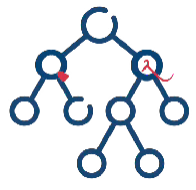
\includegraphics[height=0.9cm]{msca_logo.png}}%
  \end{center}
  \vspace{0.45cm}
  \begin{center}
    \begin{minipage}{0.1\textwidth}\centering
      \href{https://quantlet.com}{
\includegraphics[height=0.9cm]{ql_logo.png}}\end{minipage}%
    \begin{minipage}{0.78\textwidth}\centering
      {\Large\bfseries\usebeamercolor[fg]{title}\inserttitle}\par\vspace{0.25cm}
      {\large\usebeamercolor[fg]{title}\insertsubtitle}\end{minipage}%
    \begin{minipage}{0.1\textwidth}\centering
      \href{https://quantinar.com}{
\includegraphics[height=0.9cm]{qr_logo.png}}\end{minipage}
  \end{center}
  \vfill
  \hspace{0.4cm}{\bfseries\insertauthor}\par\vspace{0.12cm}
  \hspace{0.4cm}\begin{minipage}[t]{0.92\textwidth}\raggedright\footnotesize\insertinstitute\end{minipage}
  \par\vspace{0.4cm}}

% ---------------------------------------------------------------- lecture metadata
\newcommand{\nnshort}{}
\newcommand{\nnnb}{notebooks}
\newcommand{\nnrepo}{https://github.com/danpele/NEURAL_BIZ/tree/main}
% language-dependent labels (English default; \nnromanian switches to Romanian, call it before \nnlecture)
\newcommand{\txtcourse}{Neural Networks and Deep Learning}
\newcommand{\txtlecture}{Lecture}
\newcommand{\txtoutline}{Outline}
\newcommand{\txtintuition}{In one sentence:}
\newcommand{\txtjob}{In practice:}
\newcommand{\txttry}{Experiment yourself:}
\newcommand{\txtwhere}{where}
\newcommand{\txtsim}{SIMULATED DATA (teaching illustration)}
\newcommand{\txtnbsuffix}{}
\newcommand{\txtinstitute}{Bucharest University of Economic Studies (ASE), Department of Statistics and Econometrics\\
    Romanian Academy, Institute for Economic Forecasting (IPE)\\
    IDA Institute Digital Assets \textbullet\ AI4EFin \textbullet\ MSCA Digital Finance}
\newcommand{\nnromanian}{%
  \renewcommand{\txtcourse}{Rețele neuronale și deep learning}%
  \renewcommand{\txtlecture}{Cursul}%
  \renewcommand{\txtoutline}{Cuprins}%
  \renewcommand{\txtintuition}{Pe scurt:}%
  \renewcommand{\txtjob}{În practică:}%
  \renewcommand{\txttry}{Exercițiu practic:}%
  \renewcommand{\txtwhere}{unde}%
  \renewcommand{\txtsim}{DATE SIMULATE (doar pentru ilustrare)}%
  \renewcommand{\txtnbsuffix}{\string_ro}%
  \renewcommand{\txtinstitute}{Academia de Studii Economice din București (ASE), Departamentul de Statistică și Econometrie\\
    Academia Română, Institutul de Prognoză Economică (IPE)\\
    IDA Institute Digital Assets \textbullet\ AI4EFin \textbullet\ MSCA Digital Finance}}
\newcommand{\nnlecture}[2]{%
  \renewcommand{\nnshort}{\txtlecture\ #1}%
  \renewcommand{\nnnb}{notebooks/L#1\string_notebook\txtnbsuffix.ipynb}%
  \title[NN]{\txtcourse}%
  \subtitle{\txtlecture\ #1: #2}%
  \author{Prof.\ dr.\ Daniel Traian PELE}%
  \institute{\txtinstitute}%
  \date{}}

% ---------------------------------------------------------------- teaching blocks (one message per frame)
% \intuition{one plain sentence}  ->  formula with every symbol defined  ->  real-data example  ->  \manager{one line}
\newcommand{\intuition}[1]{\begin{itemize}\item {\color{MainBlue}\textbf{\txtintuition}}~#1\end{itemize}\vspace{0.6mm}}
\newcommand{\manager}[1]{\colorbox{Forest!10}{\parbox{\dimexpr\linewidth-2\fboxsep\relax}{\footnotesize
  \begin{itemize}\setlength{\itemsep}{0pt}\item \textbf{\color{Forest}\txtjob}~#1\end{itemize}}}}
% Experiment yourself: pointer to the matching notebook section
\newcommand{\tryit}[1]{{\scriptsize\href{\nnrepo/\nnnb}{%
  \raisebox{-0.15em}{
\includegraphics[height=0.85em]{ql_logo.png}}\,\textbf{\txttry}~\color{MainBlue}#1}}}
% bottom row: manager line (left) + experiment pointer (right), pinned to the bottom of the frame
\newcommand{\bottomrow}[2]{\par\vfill\noindent\begin{minipage}[b]{0.72\linewidth}#1\end{minipage}\hfill
  \begin{minipage}[b]{0.26\linewidth}\raggedleft #2\end{minipage}\par\vspace{0.5mm}}
\newcommand{\where}[1]{{\footnotesize\textbf{\txtwhere}~#1\par}}

% ---------------------------------------------------------------- helpers
% chart source line under a figure: \chartsource{Source ...; period ...}
\newcommand{\chartsource}[1]{\par\vspace{1pt}{\scriptsize\color{FooterGray}#1\par}}
% link to code: \quantlet{label}{path inside the repo}
\newcommand{\quantlet}[2]{\par\vspace{1pt}\hfill\href{\nnrepo/#2}{%
  \raisebox{-0.15em}{
\includegraphics[height=0.75em]{ql_logo.png}}\textcolor{MainBlue}{\scriptsize\ #1}}}
% inline Quantlet link for the bottom-right corner of a frame: \qlink{label}{path inside the repo}
\newcommand{\qlink}[2]{{\scriptsize\href{\nnrepo/#2}{\raisebox{-0.15em}{
\includegraphics[height=0.85em]{ql_logo.png}}\,\textcolor{MainBlue}{#1}}}}
\newcommand{\simlabel}{\colorbox{Crimson!12}{\scriptsize\bfseries\color{Crimson}\txtsim}}
\newcommand{\E}{\mathbb{E}}
\newcommand{\Var}{\operatorname{Var}}
\newcommand{\Cov}{\operatorname{Cov}}
\newcommand{\Corr}{\operatorname{Corr}}
\newcommand{\asinh}{\operatorname{asinh}}
\newcommand{\iid}{\overset{\text{i.i.d.}}{\sim}}
\newcommand{\EUR}{EUR}
% deep-learning notation (Bishop & Bishop, 2024): vectors bold lower case, matrices bold upper case
\newcommand{\R}{\mathbb{R}}
\newcommand{\vx}{\mathbf{x}}
\newcommand{\vy}{\mathbf{y}}
\newcommand{\vz}{\mathbf{z}}
\newcommand{\vh}{\mathbf{h}}
\newcommand{\vw}{\mathbf{w}}
\newcommand{\vb}{\mathbf{b}}
\newcommand{\mW}{\mathbf{W}}
\newcommand{\mX}{\mathbf{X}}
\newcommand{\btheta}{\boldsymbol{\theta}}
\newcommand{\loss}{\mathcal{L}}
\newcommand{\dataset}{\mathcal{D}}
\DeclareMathOperator*{\argmin}{arg\,min}
\DeclareMathOperator*{\argmax}{arg\,max}
\DeclareMathOperator{\softmax}{softmax}
\DeclareMathOperator{\ReLU}{ReLU}
\DeclareMathOperator{\sigm}{\sigma}

%   \nnlecture{k}{Lecture title}
% Logos live in lectures/common/logos/, charts in lectures/Lk/charts/.
% Do NOT add \hfuzz / \vfuzz / \hbadness here: overfull boxes must be fixed, not hidden.
% =============================================================================

\usetheme{default}
\setbeamersize{text margin left=7mm, text margin right=7mm}

% ---------------------------------------------------------------- packages
\usepackage[utf8]{inputenc}
\usepackage[T1]{fontenc}
\usepackage{lmodern}
\usepackage{amsmath, amssymb}
\usepackage{mathtools}
\usepackage{bm}
\usepackage{tikz}
\usetikzlibrary{arrows.meta, positioning, calc, shapes.misc}
\usepackage{booktabs}
\usepackage{array}
\usepackage{graphicx}
\usepackage{colortbl}
\usepackage{xcolor}
\usepackage{multicol}
\hypersetup{colorlinks=true, linkcolor=MainBlue, urlcolor=MainBlue, citecolor=MainBlue}
\graphicspath{{../common/logos/}}   % charts are included with their language folder: charts/en/, charts/ro/

% ---------------------------------------------------------------- colours
\definecolor{MainBlue}{RGB}{26, 58, 110}
\definecolor{IDAred}{RGB}{205, 0, 0}
\definecolor{DarkGray}{RGB}{51, 51, 51}
\definecolor{FooterGray}{RGB}{100, 100, 100}
\definecolor{BlockGray}{RGB}{236, 238, 242}
\definecolor{KeynoteGray}{RGB}{218, 218, 218}
\definecolor{Crimson}{RGB}{190, 40, 50}
\definecolor{Forest}{RGB}{30, 110, 50}
\definecolor{Bitter}{RGB}{214, 150, 20}
% chart palette (same hex values and order as lectures/common/nn_plot.py SERIES)
\definecolor{Ser1}{HTML}{2A78D6}
\definecolor{Ser2}{HTML}{EB6834}
\definecolor{Ser3}{HTML}{1BAF7A}
\definecolor{Ser4}{HTML}{EDA100}
\definecolor{Ser5}{HTML}{E87BA4}
\definecolor{Ser6}{HTML}{008300}
\definecolor{Ser7}{HTML}{6250D6}
\definecolor{Ser8}{HTML}{E34948}

\setbeamertemplate{background}{%
  \begin{tikzpicture}[remember picture, overlay]
    \shade[shading=axis, shading angle=315, top color=white, bottom color=KeynoteGray]
      (current page.south west) rectangle (current page.north east);
  \end{tikzpicture}}
\setbeamercolor{background canvas}{bg=}
\setbeamercolor{structure}{fg=MainBlue}
\setbeamercolor{normal text}{fg=DarkGray}
\setbeamercolor{title}{fg=IDAred}
\setbeamercolor{frametitle}{fg=IDAred, bg=}
\setbeamercolor{block title}{bg=MainBlue, fg=white}
\setbeamercolor{block body}{bg=BlockGray, fg=DarkGray}
\setbeamercolor{block title alerted}{bg=Crimson, fg=white}
\setbeamercolor{block body alerted}{bg=Crimson!7, fg=DarkGray}
\setbeamercolor{block title example}{bg=Forest, fg=white}
\setbeamercolor{block body example}{bg=Forest!7, fg=DarkGray}
\setbeamercolor{item}{fg=MainBlue}
\setbeamerfont{frametitle}{size=\large, series=\bfseries}
\setbeamerfont{block title}{size=\small, series=\bfseries}
\setbeamertemplate{blocks}[rounded][shadow=false]
\setbeamertemplate{itemize item}{\color{MainBlue}$\boxdot$}
\setbeamertemplate{itemize subitem}{\color{MainBlue}\scriptsize$\blacktriangleright$}
% compact two-level lists: level 1 = main point, level 2 = details (no text outside bullets)
\setbeamerfont{itemize/enumerate subbody}{size=\footnotesize}
\setlength{\leftmargini}{1.1em}
\setlength{\leftmarginii}{1.1em}
\setbeamertemplate{itemize/enumerate body begin}{\setlength{\topsep}{0pt}\setlength{\partopsep}{0pt}\setlength{\parskip}{0pt}}
\setbeamertemplate{itemize/enumerate subbody begin}{\setlength{\topsep}{0pt}\setlength{\partopsep}{0pt}\setlength{\itemsep}{0pt}\vspace{-0.4ex}}

\setbeamertemplate{enumerate item}{\color{MainBlue}\insertenumlabel.}
\setlength{\leftmargini}{1.3em}
\setlength{\leftmarginii}{1.2em}
\setbeamertemplate{navigation symbols}{}
\setbeamertemplate{section in toc}{\color{MainBlue}$\blacktriangleright$~\inserttocsection}
\setbeamertemplate{caption}{\raggedright\insertcaption\par}
% frame subtitle = precise citation line under the claim title (Weron style)
\setbeamerfont{framesubtitle}{size=\footnotesize}
\setbeamercolor{framesubtitle}{fg=FooterGray}
% outline that reappears at every section with the current section highlighted
\setbeamertemplate{section in toc shaded}[default][35]
\setbeamertemplate{subsection in toc shaded}[default][35]
\setbeamertemplate{subsection in toc}{\leavevmode\leftskip=2.2em\color{DarkGray}\small\inserttocsubsection\par}
\AtBeginSection[]{{\begin{frame}{\txtoutline}\vspace{2mm}\small
  \tableofcontents[currentsection,hideothersubsections]\end{frame}}}

% ---------------------------------------------------------------- head and foot
\setbeamertemplate{headline}{%
  \vskip10pt%
  \hbox to \paperwidth{\hskip0.5cm%
    {\small\color{FooterGray}\renewcommand{\hyperlink}[2]{##2}\insertsectionhead}%
    \hfill\textcolor{FooterGray}{\small\insertframenumber}\hskip0.5cm}%
  \vskip4pt{\color{FooterGray}\hrule height 0.4pt}}
% footer as in the other courses (MFM, SFM): course name on the left, small sparkline on the right
\setbeamertemplate{footline}{%
  {\color{FooterGray}\hrule height 0.4pt}\vskip4pt%
  \hbox to \paperwidth{\hskip0.5cm%
    \textcolor{FooterGray}{\small\txtcourse}%
    \hfill\raisebox{-0.1em}{\begin{tikzpicture}[x=0.08em, y=0.08em, line width=0.4pt]
      \draw[FooterGray] (0,3) -- (1,4) -- (2,3.5) -- (3,5) -- (4,4) -- (5,6) -- (6,5.5) -- (7,4) -- (8,5) -- (9,7) -- (10,6) -- (11,5) -- (12,6.5) -- (13,8) -- (14,7) -- (15,6) -- (16,7.5) -- (17,9) -- (18,8) -- (19,7) -- (20,8.5) -- (21,10) -- (22,9) -- (23,8) -- (24,9.5);
    \end{tikzpicture}}\hskip0.5cm}%
  \vskip6pt}

% ---------------------------------------------------------------- title page
\defbeamertemplate*{title page}{nn}[1][]{%
  \vspace{0.15cm}
  \begin{center}
    \href{https://www.ase.ro}{
\includegraphics[height=0.9cm]{ase_logo.png}}\hspace{0.3cm}%
    \href{https://ipe.ro/new}{
\includegraphics[height=0.9cm]{acad_logo.png}}\hspace{0.3cm}%
    \href{https://theida.net}{
\includegraphics[height=0.9cm]{ida_logo.png}}\hspace{0.3cm}%
    \href{https://blockchain-research-center.com}{
\includegraphics[height=0.9cm]{brc_logo.png}}\hspace{0.3cm}%
    \href{https://www.ai4efin.ase.ro}{
\includegraphics[height=0.9cm]{ai4efin_logo.png}}\hspace{0.3cm}%
    \href{https://www.digital-finance-msca.com}{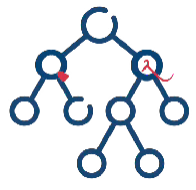
\includegraphics[height=0.9cm]{msca_logo.png}}%
  \end{center}
  \vspace{0.45cm}
  \begin{center}
    \begin{minipage}{0.1\textwidth}\centering
      \href{https://quantlet.com}{
\includegraphics[height=0.9cm]{ql_logo.png}}\end{minipage}%
    \begin{minipage}{0.78\textwidth}\centering
      {\Large\bfseries\usebeamercolor[fg]{title}\inserttitle}\par\vspace{0.25cm}
      {\large\usebeamercolor[fg]{title}\insertsubtitle}\end{minipage}%
    \begin{minipage}{0.1\textwidth}\centering
      \href{https://quantinar.com}{
\includegraphics[height=0.9cm]{qr_logo.png}}\end{minipage}
  \end{center}
  \vfill
  \hspace{0.4cm}{\bfseries\insertauthor}\par\vspace{0.12cm}
  \hspace{0.4cm}\begin{minipage}[t]{0.92\textwidth}\raggedright\footnotesize\insertinstitute\end{minipage}
  \par\vspace{0.4cm}}

% ---------------------------------------------------------------- lecture metadata
\newcommand{\nnshort}{}
\newcommand{\nnnb}{notebooks}
\newcommand{\nnrepo}{https://github.com/danpele/NEURAL_BIZ/tree/main}
% language-dependent labels (English default; \nnromanian switches to Romanian, call it before \nnlecture)
\newcommand{\txtcourse}{Neural Networks and Deep Learning}
\newcommand{\txtlecture}{Lecture}
\newcommand{\txtoutline}{Outline}
\newcommand{\txtintuition}{In one sentence:}
\newcommand{\txtjob}{In practice:}
\newcommand{\txttry}{Experiment yourself:}
\newcommand{\txtwhere}{where}
\newcommand{\txtsim}{SIMULATED DATA (teaching illustration)}
\newcommand{\txtnbsuffix}{}
\newcommand{\txtinstitute}{Bucharest University of Economic Studies (ASE), Department of Statistics and Econometrics\\
    Romanian Academy, Institute for Economic Forecasting (IPE)\\
    IDA Institute Digital Assets \textbullet\ AI4EFin \textbullet\ MSCA Digital Finance}
\newcommand{\nnromanian}{%
  \renewcommand{\txtcourse}{Rețele neuronale și deep learning}%
  \renewcommand{\txtlecture}{Cursul}%
  \renewcommand{\txtoutline}{Cuprins}%
  \renewcommand{\txtintuition}{Pe scurt:}%
  \renewcommand{\txtjob}{În practică:}%
  \renewcommand{\txttry}{Exercițiu practic:}%
  \renewcommand{\txtwhere}{unde}%
  \renewcommand{\txtsim}{DATE SIMULATE (doar pentru ilustrare)}%
  \renewcommand{\txtnbsuffix}{\string_ro}%
  \renewcommand{\txtinstitute}{Academia de Studii Economice din București (ASE), Departamentul de Statistică și Econometrie\\
    Academia Română, Institutul de Prognoză Economică (IPE)\\
    IDA Institute Digital Assets \textbullet\ AI4EFin \textbullet\ MSCA Digital Finance}}
\newcommand{\nnlecture}[2]{%
  \renewcommand{\nnshort}{\txtlecture\ #1}%
  \renewcommand{\nnnb}{notebooks/L#1\string_notebook\txtnbsuffix.ipynb}%
  \title[NN]{\txtcourse}%
  \subtitle{\txtlecture\ #1: #2}%
  \author{Prof.\ dr.\ Daniel Traian PELE}%
  \institute{\txtinstitute}%
  \date{}}

% ---------------------------------------------------------------- teaching blocks (one message per frame)
% \intuition{one plain sentence}  ->  formula with every symbol defined  ->  real-data example  ->  \manager{one line}
\newcommand{\intuition}[1]{\begin{itemize}\item {\color{MainBlue}\textbf{\txtintuition}}~#1\end{itemize}\vspace{0.6mm}}
\newcommand{\manager}[1]{\colorbox{Forest!10}{\parbox{\dimexpr\linewidth-2\fboxsep\relax}{\footnotesize
  \begin{itemize}\setlength{\itemsep}{0pt}\item \textbf{\color{Forest}\txtjob}~#1\end{itemize}}}}
% Experiment yourself: pointer to the matching notebook section
\newcommand{\tryit}[1]{{\scriptsize\href{\nnrepo/\nnnb}{%
  \raisebox{-0.15em}{
\includegraphics[height=0.85em]{ql_logo.png}}\,\textbf{\txttry}~\color{MainBlue}#1}}}
% bottom row: manager line (left) + experiment pointer (right), pinned to the bottom of the frame
\newcommand{\bottomrow}[2]{\par\vfill\noindent\begin{minipage}[b]{0.72\linewidth}#1\end{minipage}\hfill
  \begin{minipage}[b]{0.26\linewidth}\raggedleft #2\end{minipage}\par\vspace{0.5mm}}
\newcommand{\where}[1]{{\footnotesize\textbf{\txtwhere}~#1\par}}

% ---------------------------------------------------------------- helpers
% chart source line under a figure: \chartsource{Source ...; period ...}
\newcommand{\chartsource}[1]{\par\vspace{1pt}{\scriptsize\color{FooterGray}#1\par}}
% link to code: \quantlet{label}{path inside the repo}
\newcommand{\quantlet}[2]{\par\vspace{1pt}\hfill\href{\nnrepo/#2}{%
  \raisebox{-0.15em}{
\includegraphics[height=0.75em]{ql_logo.png}}\textcolor{MainBlue}{\scriptsize\ #1}}}
% inline Quantlet link for the bottom-right corner of a frame: \qlink{label}{path inside the repo}
\newcommand{\qlink}[2]{{\scriptsize\href{\nnrepo/#2}{\raisebox{-0.15em}{
\includegraphics[height=0.85em]{ql_logo.png}}\,\textcolor{MainBlue}{#1}}}}
\newcommand{\simlabel}{\colorbox{Crimson!12}{\scriptsize\bfseries\color{Crimson}\txtsim}}
\newcommand{\E}{\mathbb{E}}
\newcommand{\Var}{\operatorname{Var}}
\newcommand{\Cov}{\operatorname{Cov}}
\newcommand{\Corr}{\operatorname{Corr}}
\newcommand{\asinh}{\operatorname{asinh}}
\newcommand{\iid}{\overset{\text{i.i.d.}}{\sim}}
\newcommand{\EUR}{EUR}
% deep-learning notation (Bishop & Bishop, 2024): vectors bold lower case, matrices bold upper case
\newcommand{\R}{\mathbb{R}}
\newcommand{\vx}{\mathbf{x}}
\newcommand{\vy}{\mathbf{y}}
\newcommand{\vz}{\mathbf{z}}
\newcommand{\vh}{\mathbf{h}}
\newcommand{\vw}{\mathbf{w}}
\newcommand{\vb}{\mathbf{b}}
\newcommand{\mW}{\mathbf{W}}
\newcommand{\mX}{\mathbf{X}}
\newcommand{\btheta}{\boldsymbol{\theta}}
\newcommand{\loss}{\mathcal{L}}
\newcommand{\dataset}{\mathcal{D}}
\DeclareMathOperator*{\argmin}{arg\,min}
\DeclareMathOperator*{\argmax}{arg\,max}
\DeclareMathOperator{\softmax}{softmax}
\DeclareMathOperator{\ReLU}{ReLU}
\DeclareMathOperator{\sigm}{\sigma}

%   \nnlecture{k}{Lecture title}
% Logos live in lectures/common/logos/, charts in lectures/Lk/charts/.
% Do NOT add \hfuzz / \vfuzz / \hbadness here: overfull boxes must be fixed, not hidden.
% =============================================================================

\usetheme{default}
\setbeamersize{text margin left=7mm, text margin right=7mm}

% ---------------------------------------------------------------- packages
\usepackage[utf8]{inputenc}
\usepackage[T1]{fontenc}
\usepackage{lmodern}
\usepackage{amsmath, amssymb}
\usepackage{mathtools}
\usepackage{bm}
\usepackage{tikz}
\usetikzlibrary{arrows.meta, positioning, calc, shapes.misc}
\usepackage{booktabs}
\usepackage{array}
\usepackage{graphicx}
\usepackage{colortbl}
\usepackage{xcolor}
\usepackage{multicol}
\hypersetup{colorlinks=true, linkcolor=MainBlue, urlcolor=MainBlue, citecolor=MainBlue}
\graphicspath{{../common/logos/}}   % charts are included with their language folder: charts/en/, charts/ro/

% ---------------------------------------------------------------- colours
\definecolor{MainBlue}{RGB}{26, 58, 110}
\definecolor{IDAred}{RGB}{205, 0, 0}
\definecolor{DarkGray}{RGB}{51, 51, 51}
\definecolor{FooterGray}{RGB}{100, 100, 100}
\definecolor{BlockGray}{RGB}{236, 238, 242}
\definecolor{KeynoteGray}{RGB}{218, 218, 218}
\definecolor{Crimson}{RGB}{190, 40, 50}
\definecolor{Forest}{RGB}{30, 110, 50}
\definecolor{Bitter}{RGB}{214, 150, 20}
% chart palette (same hex values and order as lectures/common/nn_plot.py SERIES)
\definecolor{Ser1}{HTML}{2A78D6}
\definecolor{Ser2}{HTML}{EB6834}
\definecolor{Ser3}{HTML}{1BAF7A}
\definecolor{Ser4}{HTML}{EDA100}
\definecolor{Ser5}{HTML}{E87BA4}
\definecolor{Ser6}{HTML}{008300}
\definecolor{Ser7}{HTML}{6250D6}
\definecolor{Ser8}{HTML}{E34948}

\setbeamertemplate{background}{%
  \begin{tikzpicture}[remember picture, overlay]
    \shade[shading=axis, shading angle=315, top color=white, bottom color=KeynoteGray]
      (current page.south west) rectangle (current page.north east);
  \end{tikzpicture}}
\setbeamercolor{background canvas}{bg=}
\setbeamercolor{structure}{fg=MainBlue}
\setbeamercolor{normal text}{fg=DarkGray}
\setbeamercolor{title}{fg=IDAred}
\setbeamercolor{frametitle}{fg=IDAred, bg=}
\setbeamercolor{block title}{bg=MainBlue, fg=white}
\setbeamercolor{block body}{bg=BlockGray, fg=DarkGray}
\setbeamercolor{block title alerted}{bg=Crimson, fg=white}
\setbeamercolor{block body alerted}{bg=Crimson!7, fg=DarkGray}
\setbeamercolor{block title example}{bg=Forest, fg=white}
\setbeamercolor{block body example}{bg=Forest!7, fg=DarkGray}
\setbeamercolor{item}{fg=MainBlue}
\setbeamerfont{frametitle}{size=\large, series=\bfseries}
\setbeamerfont{block title}{size=\small, series=\bfseries}
\setbeamertemplate{blocks}[rounded][shadow=false]
\setbeamertemplate{itemize item}{\color{MainBlue}$\boxdot$}
\setbeamertemplate{itemize subitem}{\color{MainBlue}\scriptsize$\blacktriangleright$}
% compact two-level lists: level 1 = main point, level 2 = details (no text outside bullets)
\setbeamerfont{itemize/enumerate subbody}{size=\footnotesize}
\setlength{\leftmargini}{1.1em}
\setlength{\leftmarginii}{1.1em}
\setbeamertemplate{itemize/enumerate body begin}{\setlength{\topsep}{0pt}\setlength{\partopsep}{0pt}\setlength{\parskip}{0pt}}
\setbeamertemplate{itemize/enumerate subbody begin}{\setlength{\topsep}{0pt}\setlength{\partopsep}{0pt}\setlength{\itemsep}{0pt}\vspace{-0.4ex}}

\setbeamertemplate{enumerate item}{\color{MainBlue}\insertenumlabel.}
\setlength{\leftmargini}{1.3em}
\setlength{\leftmarginii}{1.2em}
\setbeamertemplate{navigation symbols}{}
\setbeamertemplate{section in toc}{\color{MainBlue}$\blacktriangleright$~\inserttocsection}
\setbeamertemplate{caption}{\raggedright\insertcaption\par}
% frame subtitle = precise citation line under the claim title (Weron style)
\setbeamerfont{framesubtitle}{size=\footnotesize}
\setbeamercolor{framesubtitle}{fg=FooterGray}
% outline that reappears at every section with the current section highlighted
\setbeamertemplate{section in toc shaded}[default][35]
\setbeamertemplate{subsection in toc shaded}[default][35]
\setbeamertemplate{subsection in toc}{\leavevmode\leftskip=2.2em\color{DarkGray}\small\inserttocsubsection\par}
\AtBeginSection[]{{\begin{frame}{\txtoutline}\vspace{2mm}\small
  \tableofcontents[currentsection,hideothersubsections]\end{frame}}}

% ---------------------------------------------------------------- head and foot
\setbeamertemplate{headline}{%
  \vskip10pt%
  \hbox to \paperwidth{\hskip0.5cm%
    {\small\color{FooterGray}\renewcommand{\hyperlink}[2]{##2}\insertsectionhead}%
    \hfill\textcolor{FooterGray}{\small\insertframenumber}\hskip0.5cm}%
  \vskip4pt{\color{FooterGray}\hrule height 0.4pt}}
% footer as in the other courses (MFM, SFM): course name on the left, small sparkline on the right
\setbeamertemplate{footline}{%
  {\color{FooterGray}\hrule height 0.4pt}\vskip4pt%
  \hbox to \paperwidth{\hskip0.5cm%
    \textcolor{FooterGray}{\small\txtcourse}%
    \hfill\raisebox{-0.1em}{\begin{tikzpicture}[x=0.08em, y=0.08em, line width=0.4pt]
      \draw[FooterGray] (0,3) -- (1,4) -- (2,3.5) -- (3,5) -- (4,4) -- (5,6) -- (6,5.5) -- (7,4) -- (8,5) -- (9,7) -- (10,6) -- (11,5) -- (12,6.5) -- (13,8) -- (14,7) -- (15,6) -- (16,7.5) -- (17,9) -- (18,8) -- (19,7) -- (20,8.5) -- (21,10) -- (22,9) -- (23,8) -- (24,9.5);
    \end{tikzpicture}}\hskip0.5cm}%
  \vskip6pt}

% ---------------------------------------------------------------- title page
\defbeamertemplate*{title page}{nn}[1][]{%
  \vspace{0.15cm}
  \begin{center}
    \href{https://www.ase.ro}{
\includegraphics[height=0.9cm]{ase_logo.png}}\hspace{0.3cm}%
    \href{https://ipe.ro/new}{
\includegraphics[height=0.9cm]{acad_logo.png}}\hspace{0.3cm}%
    \href{https://theida.net}{
\includegraphics[height=0.9cm]{ida_logo.png}}\hspace{0.3cm}%
    \href{https://blockchain-research-center.com}{
\includegraphics[height=0.9cm]{brc_logo.png}}\hspace{0.3cm}%
    \href{https://www.ai4efin.ase.ro}{
\includegraphics[height=0.9cm]{ai4efin_logo.png}}\hspace{0.3cm}%
    \href{https://www.digital-finance-msca.com}{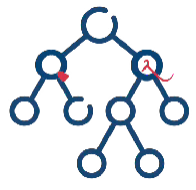
\includegraphics[height=0.9cm]{msca_logo.png}}%
  \end{center}
  \vspace{0.45cm}
  \begin{center}
    \begin{minipage}{0.1\textwidth}\centering
      \href{https://quantlet.com}{
\includegraphics[height=0.9cm]{ql_logo.png}}\end{minipage}%
    \begin{minipage}{0.78\textwidth}\centering
      {\Large\bfseries\usebeamercolor[fg]{title}\inserttitle}\par\vspace{0.25cm}
      {\large\usebeamercolor[fg]{title}\insertsubtitle}\end{minipage}%
    \begin{minipage}{0.1\textwidth}\centering
      \href{https://quantinar.com}{
\includegraphics[height=0.9cm]{qr_logo.png}}\end{minipage}
  \end{center}
  \vfill
  \hspace{0.4cm}{\bfseries\insertauthor}\par\vspace{0.12cm}
  \hspace{0.4cm}\begin{minipage}[t]{0.92\textwidth}\raggedright\footnotesize\insertinstitute\end{minipage}
  \par\vspace{0.4cm}}

% ---------------------------------------------------------------- lecture metadata
\newcommand{\nnshort}{}
\newcommand{\nnnb}{notebooks}
\newcommand{\nnrepo}{https://github.com/danpele/NEURAL_BIZ/tree/main}
% language-dependent labels (English default; \nnromanian switches to Romanian, call it before \nnlecture)
\newcommand{\txtcourse}{Neural Networks and Deep Learning}
\newcommand{\txtlecture}{Lecture}
\newcommand{\txtoutline}{Outline}
\newcommand{\txtintuition}{In one sentence:}
\newcommand{\txtjob}{In practice:}
\newcommand{\txttry}{Experiment yourself:}
\newcommand{\txtwhere}{where}
\newcommand{\txtsim}{SIMULATED DATA (teaching illustration)}
\newcommand{\txtnbsuffix}{}
\newcommand{\txtinstitute}{Bucharest University of Economic Studies (ASE), Department of Statistics and Econometrics\\
    Romanian Academy, Institute for Economic Forecasting (IPE)\\
    IDA Institute Digital Assets \textbullet\ AI4EFin \textbullet\ MSCA Digital Finance}
\newcommand{\nnromanian}{%
  \renewcommand{\txtcourse}{Rețele neuronale și deep learning}%
  \renewcommand{\txtlecture}{Cursul}%
  \renewcommand{\txtoutline}{Cuprins}%
  \renewcommand{\txtintuition}{Pe scurt:}%
  \renewcommand{\txtjob}{În practică:}%
  \renewcommand{\txttry}{Exercițiu practic:}%
  \renewcommand{\txtwhere}{unde}%
  \renewcommand{\txtsim}{DATE SIMULATE (doar pentru ilustrare)}%
  \renewcommand{\txtnbsuffix}{\string_ro}%
  \renewcommand{\txtinstitute}{Academia de Studii Economice din București (ASE), Departamentul de Statistică și Econometrie\\
    Academia Română, Institutul de Prognoză Economică (IPE)\\
    IDA Institute Digital Assets \textbullet\ AI4EFin \textbullet\ MSCA Digital Finance}}
\newcommand{\nnlecture}[2]{%
  \renewcommand{\nnshort}{\txtlecture\ #1}%
  \renewcommand{\nnnb}{notebooks/L#1\string_notebook\txtnbsuffix.ipynb}%
  \title[NN]{\txtcourse}%
  \subtitle{\txtlecture\ #1: #2}%
  \author{Prof.\ dr.\ Daniel Traian PELE}%
  \institute{\txtinstitute}%
  \date{}}

% ---------------------------------------------------------------- teaching blocks (one message per frame)
% \intuition{one plain sentence}  ->  formula with every symbol defined  ->  real-data example  ->  \manager{one line}
\newcommand{\intuition}[1]{\begin{itemize}\item {\color{MainBlue}\textbf{\txtintuition}}~#1\end{itemize}\vspace{0.6mm}}
\newcommand{\manager}[1]{\colorbox{Forest!10}{\parbox{\dimexpr\linewidth-2\fboxsep\relax}{\footnotesize
  \begin{itemize}\setlength{\itemsep}{0pt}\item \textbf{\color{Forest}\txtjob}~#1\end{itemize}}}}
% Experiment yourself: pointer to the matching notebook section
\newcommand{\tryit}[1]{{\scriptsize\href{\nnrepo/\nnnb}{%
  \raisebox{-0.15em}{
\includegraphics[height=0.85em]{ql_logo.png}}\,\textbf{\txttry}~\color{MainBlue}#1}}}
% bottom row: manager line (left) + experiment pointer (right), pinned to the bottom of the frame
\newcommand{\bottomrow}[2]{\par\vfill\noindent\begin{minipage}[b]{0.72\linewidth}#1\end{minipage}\hfill
  \begin{minipage}[b]{0.26\linewidth}\raggedleft #2\end{minipage}\par\vspace{0.5mm}}
\newcommand{\where}[1]{{\footnotesize\textbf{\txtwhere}~#1\par}}

% ---------------------------------------------------------------- helpers
% chart source line under a figure: \chartsource{Source ...; period ...}
\newcommand{\chartsource}[1]{\par\vspace{1pt}{\scriptsize\color{FooterGray}#1\par}}
% link to code: \quantlet{label}{path inside the repo}
\newcommand{\quantlet}[2]{\par\vspace{1pt}\hfill\href{\nnrepo/#2}{%
  \raisebox{-0.15em}{
\includegraphics[height=0.75em]{ql_logo.png}}\textcolor{MainBlue}{\scriptsize\ #1}}}
% inline Quantlet link for the bottom-right corner of a frame: \qlink{label}{path inside the repo}
\newcommand{\qlink}[2]{{\scriptsize\href{\nnrepo/#2}{\raisebox{-0.15em}{
\includegraphics[height=0.85em]{ql_logo.png}}\,\textcolor{MainBlue}{#1}}}}
\newcommand{\simlabel}{\colorbox{Crimson!12}{\scriptsize\bfseries\color{Crimson}\txtsim}}
\newcommand{\E}{\mathbb{E}}
\newcommand{\Var}{\operatorname{Var}}
\newcommand{\Cov}{\operatorname{Cov}}
\newcommand{\Corr}{\operatorname{Corr}}
\newcommand{\asinh}{\operatorname{asinh}}
\newcommand{\iid}{\overset{\text{i.i.d.}}{\sim}}
\newcommand{\EUR}{EUR}
% deep-learning notation (Bishop & Bishop, 2024): vectors bold lower case, matrices bold upper case
\newcommand{\R}{\mathbb{R}}
\newcommand{\vx}{\mathbf{x}}
\newcommand{\vy}{\mathbf{y}}
\newcommand{\vz}{\mathbf{z}}
\newcommand{\vh}{\mathbf{h}}
\newcommand{\vw}{\mathbf{w}}
\newcommand{\vb}{\mathbf{b}}
\newcommand{\mW}{\mathbf{W}}
\newcommand{\mX}{\mathbf{X}}
\newcommand{\btheta}{\boldsymbol{\theta}}
\newcommand{\loss}{\mathcal{L}}
\newcommand{\dataset}{\mathcal{D}}
\DeclareMathOperator*{\argmin}{arg\,min}
\DeclareMathOperator*{\argmax}{arg\,max}
\DeclareMathOperator{\softmax}{softmax}
\DeclareMathOperator{\ReLU}{ReLU}
\DeclareMathOperator{\sigm}{\sigma}

\nnlecture{14}{Multimodal and vision-language models; synthesis of the course}
\begin{document}
{\setbeamertemplate{headline}{}\setbeamertemplate{footline}{}
\begin{frame}\titlepage\end{frame}}
% END-FRONT-MATTER

\begin{frame}{Learning objectives}
\small
\begin{itemize}\setlength{\itemsep}{4pt}
  \item Explain how a vision transformer turns an image into tokens and where its attention goes, on real satellite images.
  \item Write the contrastive loss of contrastive language--image pre-training (CLIP), use it as a zero-shot classifier and compare it with a convolutional neural network (CNN) trained on labelled images.
  \item Describe how vision-language models connect an image encoder to a language model, and test what they can read in charts and tables.
  \item Synthesise the course: choose a model for a business problem, from logistic regression to foundation models, with the right evaluation.
\end{itemize}
\end{frame}

% BEGIN-ABBR

\begin{frame}{Abbreviations}
\small
\vspace{-1mm}\begin{columns}[T,onlytextwidth]
\begin{column}{0.49\textwidth}{\scriptsize\renewcommand{\arraystretch}{0.96}\begin{tabular}{@{}>{\bfseries}l@{\ \ }p{0.74\linewidth}@{}}ASE & Bucharest University of Economic Studies\\
AUC & area under the receiver operating characteristic curve\\
CLIP & contrastive language--image pre-training\\
CNN & convolutional neural network\\
ECB & European Central Bank\\
ESG & environmental, social and governance\\
GAN & generative adversarial network\\
GNN & graph neural network\\
GPT & generative pre-trained transformer\\
ICBE & International Conference on Business Excellence\\
InfoNCE & information noise-contrastive estimation loss\\
IPE & Institute for Economic Forecasting, Romanian Academy\\
LLaVA & large language and vision assistant\\
LLM & large language model\\\end{tabular}}\end{column}
\begin{column}{0.49\textwidth}{\scriptsize\renewcommand{\arraystretch}{0.96}\begin{tabular}{@{}>{\bfseries}l@{\ \ }p{0.74\linewidth}@{}}LSTM & long short-term memory network\\
MLP & multilayer perceptron\\
OCR & optical character recognition\\
RAG & retrieval-augmented generation\\
RGB & red, green, blue (colour channels)\\
RL & reinforcement learning\\
ROC & receiver operating characteristic\\
SHAP & Shapley additive explanations\\
VAE & variational autoencoder\\
VaR & Value-at-Risk\\
ViT & vision transformer\\
VLM & vision-language model\\
XAI & explainable artificial intelligence\\\end{tabular}}\end{column}
\end{columns}
\end{frame}

% END-ABBR


\section{Why multimodal models}

\begin{frame}{Images, documents and charts as business data}
\small
\begin{itemize}\setlength{\itemsep}{3pt}
  \item \textbf{Satellite and aerial images}
    \begin{itemize}\setlength{\itemsep}{0pt}
      \item Crop monitoring for agricultural credit and insurance; land use for environmental, social and governance (ESG) reporting
    \end{itemize}
  \item \textbf{Documents}
    \begin{itemize}\setlength{\itemsep}{0pt}
      \item Scanned contracts, invoices, annual reports: text, tables and layout together
    \end{itemize}
  \item \textbf{Charts}
    \begin{itemize}\setlength{\itemsep}{0pt}
      \item Analysts read price charts; can a model read them, and should it, when the numbers exist?
    \end{itemize}
  \item \textbf{This lecture}
    \begin{itemize}\setlength{\itemsep}{0pt}
      \item CLIP and a vision-language model (VLM), measured on real images
    \end{itemize}
\end{itemize}
\par\vfill\noindent{\scriptsize\color{FooterGray}(Radford et al., 2021; Bishop \& Bishop, 2024)}\par\vspace{0.5mm}
\end{frame}

\begin{frame}{Business application: land use for credit, insurance and ESG}
\small
\begin{itemize}\setlength{\itemsep}{3pt}
  \item \textbf{Agricultural credit}
    \begin{itemize}\setlength{\itemsep}{0pt}
      \item A bank checks that the financed plots are cropland and stay cropland over the season
    \end{itemize}
  \item \textbf{Insurance}
    \begin{itemize}\setlength{\itemsep}{0pt}
      \item Flood and drought claims are compared with images before and after the event
    \end{itemize}
  \item \textbf{ESG reporting}
    \begin{itemize}\setlength{\itemsep}{0pt}
      \item Forest cover and industrial sites around the assets of a portfolio
    \end{itemize}
  \item \textbf{The data problem}
    \begin{itemize}\setlength{\itemsep}{0pt}
      \item Images are free (Sentinel-2 every few days), labels are expensive: hence zero-shot and few-shot models
    \end{itemize}
\end{itemize}
\par\vfill\noindent{\scriptsize\color{FooterGray}(Helber et al., 2019)}\par\vspace{0.5mm}
\end{frame}

\begin{frame}{Real data only: satellite images, market charts, yield-curve tables}
\small
{\footnotesize\renewcommand{\arraystretch}{1.05}\setlength{\tabcolsep}{4pt}
\begin{tabular}{@{}p{0.3\textwidth}p{0.3\textwidth}p{0.33\textwidth}@{}}\toprule
Data & Size & Task \\ \midrule
EuroSAT: Sentinel-2 images of Europe, red, green, blue (RGB) channels & 27\,000 images\, 64$\times$64 pixels\, 10 classes & land-use classification: zero-shot, few-shot, full training \\
S\&P 500 daily closes (Yahoo Finance), rendered as chart images & 945 windows of 120 days & market regime from the picture vs from the numbers \\
Euro area AAA yield curve, European Central Bank (ECB) & 60 tables rendered as images & can a VLM read a number from a table? \\
\bottomrule\end{tabular}}
\par\vspace{0.5mm}{\scriptsize \begin{itemize}\setlength{\itemsep}{0pt}
  \item EuroSAT split 80/20 stratified (seed 20261108): 21\,600 training and 5\,400 test images.
\end{itemize}}
\par\vfill\noindent{\scriptsize\color{FooterGray}(Helber et al., 2019)}\par\vspace{0.5mm}
\end{frame}


\section{Vision transformers}

\begin{frame}{A vision transformer reads an image as a sequence of patches}
\footnotesize
\intuition{cut the image into 16$\times$16 patches, flatten each patch into a vector, and treat the vectors as words.}
\begin{columns}[T,onlytextwidth]
\begin{column}{0.53\textwidth}
\[ \mathbf z_0=\big[\mathbf x_{\text{cls}};\ \mathbf E\mathbf p_1;\ \dots;\ \mathbf E\mathbf p_{196}\big]+\mathbf E_{\text{pos}},\quad \mathbf p_j\in\R^{16\cdot16\cdot3} \]\[ \mathbf z_\ell=\mathbf z_{\ell-1}+\mathrm{MSA}(\mathrm{LN}(\mathbf z_{\ell-1})),\ \ \mathbf z_\ell\leftarrow\mathbf z_\ell+\mathrm{MLP}(\mathrm{LN}(\mathbf z_\ell)) \]{\footnotesize\begin{itemize}\setlength{\itemsep}{0pt}
  \item \textbf{\txtwhere}
    \begin{itemize}\setlength{\itemsep}{0pt}
      \item $224\times224$ image = $14\times14$ = 196 patches + one class token = 197 tokens
      \item $\mathbf E$ = linear patch embedding (width 768)
      \item Multi-head self-attention with 12 heads, 12 layers
      \item Layer normalisation
      \item Multilayer perceptron (MLP).
    \end{itemize}
\end{itemize}\par}
\end{column}
\begin{column}{0.44\textwidth}
\begin{itemize}\setlength{\itemsep}{2pt}
  \item \textbf{Vision transformer (ViT)}: no convolution
    \begin{itemize}\setlength{\itemsep}{0pt}
      \item Locality must be learned from data.
    \end{itemize}
  \item \textbf{Hence the need for huge pre-training}: CLIP saw 400 million image--text pairs.
\end{itemize}
\end{column}
\end{columns}
\par\vfill\manager{with few labelled images, a pre-trained ViT beats a ViT trained from scratch by a wide margin.}\par\vspace{0.5mm}
\par\vfill\noindent{\scriptsize\color{FooterGray}(Dosovitskiy et al., 2021)}\hfill\tryit{notebook \S1}\par\vspace{0.5mm}
\end{frame}

\begin{frame}{Patches and attention on real EuroSAT images}
\small
\intuition{top: the 14$\times$14 patch grid; bottom: where the class token looks, averaged over all layers.}
\begin{center}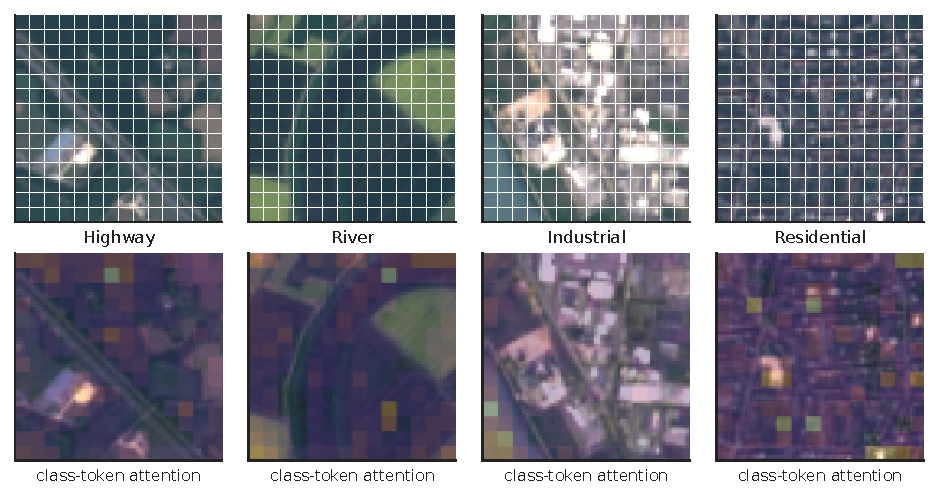
\includegraphics[width=\textwidth,height=0.475\textheight,keepaspectratio]{charts/en/vit_patches_attention.pdf}\end{center}\vspace{-3mm}
\chartsource{Source: EuroSAT, Sentinel-2 images (Helber et al., 2019). Data: 4 test images upscaled to 224 x 224 pixels = 14 x 14 patches of 16 x 16; model CLIP ViT-B/16.}
\vspace{0.5mm}
\begin{itemize}\setlength{\itemsep}{0pt}
  \item Attention rollout: $\tilde{\mathbf A}=\prod_{\ell}(\frac12\bar{\mathbf A}_\ell+\frac12\mathbf I)$, row of the class token
    \begin{itemize}\setlength{\itemsep}{0pt}
      \item $\bar{\mathbf A}_\ell$ = attention of layer $\ell$ averaged over heads.
    \end{itemize}
\end{itemize}
\par\vfill\noindent{\scriptsize\color{FooterGray}(Abnar \& Zuidema, 2020)}\hfill\qlink{NN\_L14\_vit\_patches\_attention}{Quantlets/L14/NN_L14_vit_patches_attention}\par\vspace{0.5mm}
\end{frame}


\section{CLIP: images and text in one space}

\begin{frame}{CLIP learns by matching images with their captions}
\footnotesize
\intuition{in a batch of $n$ image--caption pairs, each image must find its own caption, and vice versa.}
\begin{columns}[T,onlytextwidth]
\begin{column}{0.58\textwidth}
\[ s_{ij}=\frac{\mathbf u_i^{\top}\mathbf v_j}{\tau},\quad \mathbf u_i=\frac{f(I_i)}{\lVert f(I_i)\rVert},\ \mathbf v_j=\frac{g(T_j)}{\lVert g(T_j)\rVert} \]\[ \loss=-\frac{1}{2n}\sum_{i=1}^{n}\Big[\log\frac{e^{s_{ii}}}{\sum_{j}e^{s_{ij}}}+\log\frac{e^{s_{ii}}}{\sum_{j}e^{s_{ji}}}\Big] \]{\footnotesize\begin{itemize}\setlength{\itemsep}{0pt}
  \item \textbf{\txtwhere}
    \begin{itemize}\setlength{\itemsep}{0pt}
      \item $f$ = image encoder (ViT)
      \item $g$ = text encoder (transformer)
      \item $\tau$ = learned temperature
      \item Information noise-contrastive estimation (InfoNCE) loss in both directions.
    \end{itemize}
\end{itemize}\par}
\end{column}
\begin{column}{0.39\textwidth}
\begin{itemize}\setlength{\itemsep}{2pt}
  \item \textbf{ViT-B/32}: 151.3 million parameters
    \begin{itemize}\setlength{\itemsep}{0pt}
      \item \textbf{ViT-B/16}: 149.6 million.
    \end{itemize}
  \item \textbf{No class labels} were used in training: only captions from the web.
\end{itemize}
\end{column}
\end{columns}
\par\vfill\manager{one embedding space for images and text enables search, zero-shot labels and retrieval for retrieval-augmented generation (RAG).}\par\vspace{0.5mm}
\par\vfill\noindent{\scriptsize\color{FooterGray}(Radford et al., 2021; Oord et al., 2018)}\par\vspace{0.5mm}
\end{frame}

\begin{frame}{Zero-shot classification: the class names become the classifier}
\footnotesize
\intuition{embed one sentence per class, embed the image, and pick the closest sentence.}
\begin{columns}[T,onlytextwidth]
\begin{column}{0.53\textwidth}
\[ \mathbf w_c=\mathrm{norm}\Big(\frac{1}{M}\sum_{m=1}^{M}g\big(\text{template}_m(c)\big)\Big) \]\[ \hat c(I)=\argmax_c\ \mathbf u(I)^{\top}\mathbf w_c \]{\footnotesize\begin{itemize}\setlength{\itemsep}{0pt}
  \item \textbf{\txtwhere}
    \begin{itemize}\setlength{\itemsep}{0pt}
      \item Template$_m$ = sentence such as ``a satellite photo of \{class\}.''
      \item $M$ = 1 or 5 templates (prompt ensemble)
      \item Class descriptions as in Radford et al.\ (2021).
    \end{itemize}
\end{itemize}\par}
\end{column}
\begin{column}{0.44\textwidth}
\begin{itemize}\setlength{\itemsep}{2pt}
  \item \textbf{Best zero-shot}: CLIP ViT-B/16, 56.4\,\% on 5\,400 test images, without one labelled example.
  \item \textbf{Chance} with 10 classes: 10\,\%.
\end{itemize}
\end{column}
\end{columns}
\par\vfill\manager{the weight vectors are written in English, so a domain expert can edit the classifier without retraining.}\par\vspace{0.5mm}
\par\vfill\noindent{\scriptsize\color{FooterGray}(Radford et al., 2021)}\hfill\tryit{notebook \S2}\par\vspace{0.5mm}
\end{frame}

\begin{frame}{The words in the prompt change zero-shot accuracy}
\small
\intuition{telling CLIP that the image is a satellite photo is worth more than a bigger model.}
\begin{center}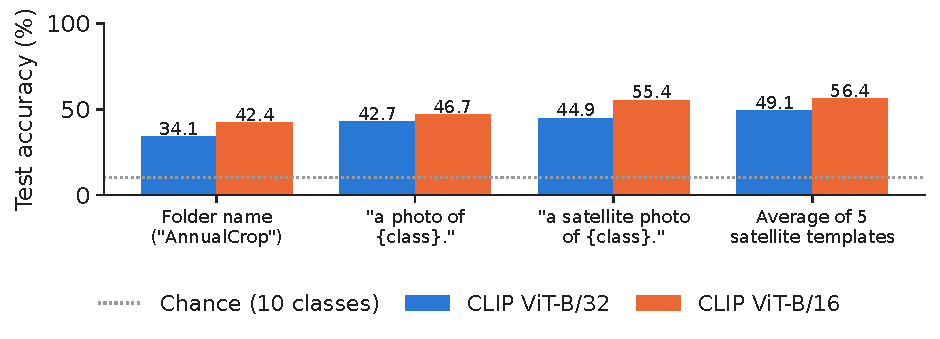
\includegraphics[width=\textwidth,height=0.475\textheight,keepaspectratio]{charts/en/zeroshot_prompts.pdf}\end{center}\vspace{-3mm}
\chartsource{Source: EuroSAT, Sentinel-2 images (Helber et al., 2019). Data: 5400 test images, no training.}
\vspace{0.5mm}
\begin{itemize}\setlength{\itemsep}{0pt}
  \item ViT-B/16: folder name 42.4\,\%, ``a satellite photo of'' 55.4\,\%, 5-template ensemble 56.4\,\%
    \begin{itemize}\setlength{\itemsep}{0pt}
      \item ViT-B/32 ensemble 49.1\,\%.
    \end{itemize}
\end{itemize}
\par\vfill\manager{prompt wording is a hyper-parameter: select it on validation images, then freeze it.}\par\vspace{0.5mm}
\par\vfill\noindent{\scriptsize\color{FooterGray}}\hfill\qlink{NN\_L14\_zeroshot\_prompts}{Quantlets/L14/NN_L14_zeroshot_prompts}\par\vspace{0.5mm}
\end{frame}

\begin{frame}{Zero-shot predictions on eight random test images}
\small
\intuition{green: correct; red: wrong; the percentage is the softmax probability of the chosen class.}
\begin{center}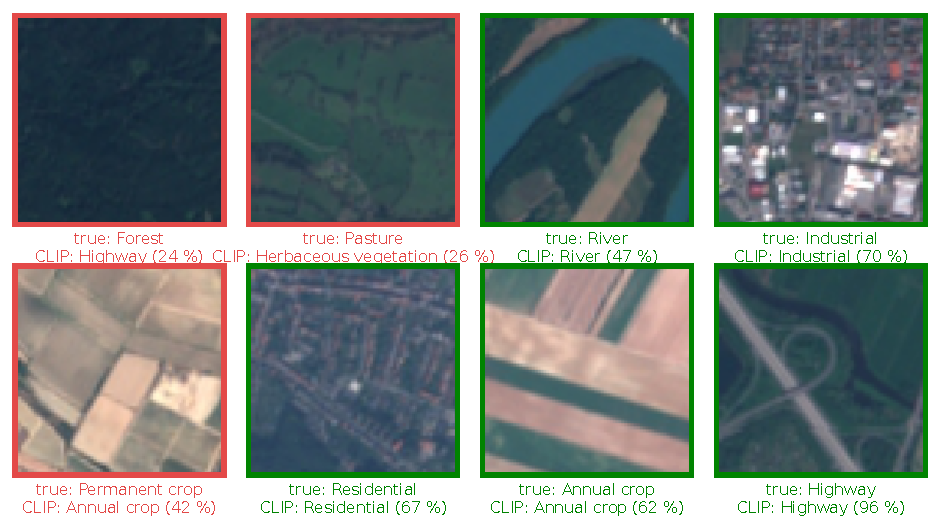
\includegraphics[width=\textwidth,height=0.563\textheight,keepaspectratio]{charts/en/zeroshot_examples.pdf}\end{center}\vspace{-3mm}
\chartsource{Source: EuroSAT, Sentinel-2 images (Helber et al., 2019). Data: 8 random test images (seeded); green = correct, red = wrong.}
\vspace{0.5mm}
\begin{itemize}\setlength{\itemsep}{0pt}
  \item 5 of 8 correct in this sample.
\end{itemize}
\par\vfill\noindent{\scriptsize\color{FooterGray}}\hfill\qlink{NN\_L14\_zeroshot\_examples}{Quantlets/L14/NN_L14_zeroshot_examples}\par\vspace{0.5mm}
\end{frame}

\begin{frame}{Where zero-shot fails: similar-looking land uses}
\small
\intuition{rows: true class; columns: predicted class; each row sums to 100\,\%.}
\begin{center}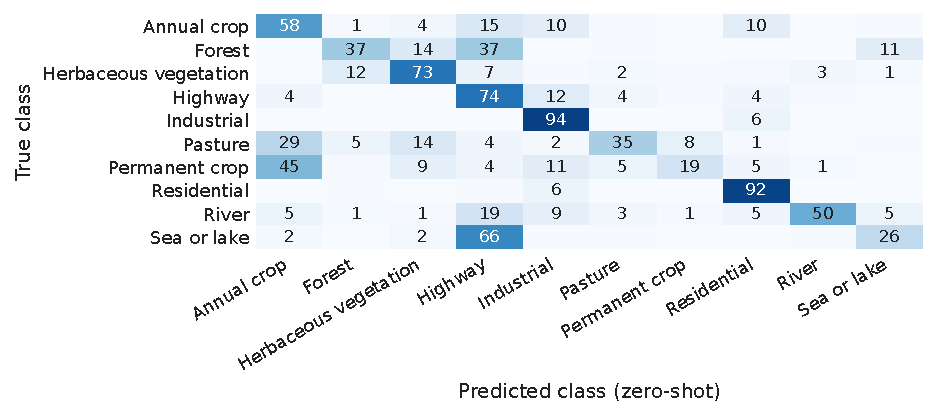
\includegraphics[width=\textwidth,height=0.524\textheight,keepaspectratio]{charts/en/zeroshot_confusion.pdf}\end{center}\vspace{-3mm}
\chartsource{Source: EuroSAT, Sentinel-2 images (Helber et al., 2019). Data: 5400 test images; row percentages.}
\vspace{0.5mm}
\begin{itemize}\setlength{\itemsep}{0pt}
  \item Best class: industrial (93.6\,\%)
    \begin{itemize}\setlength{\itemsep}{0pt}
      \item Worst: permanent crop (18.6\,\%)
      \item Largest confusion: 399 of 600 sea or lake images called highway.
    \end{itemize}
\end{itemize}
\par\vfill\noindent{\scriptsize\color{FooterGray}}\hfill\qlink{NN\_L14\_zeroshot\_confusion}{Quantlets/L14/NN_L14_zeroshot_confusion}\par\vspace{0.5mm}
\end{frame}

\begin{frame}{Text-to-image search with the same embeddings}
\small
\intuition{rank all test images by their similarity to a sentence; a bank can find flooded fields or new buildings without labels.}
\vspace{-1mm}\[ \mathrm{P@}k(c)=\frac{1}{k}\sum_{j\in\mathrm{top}_k(\mathbf w_c)}\mathbb 1\{y_j=c\},\quad \mathrm{top}_k(\mathbf w_c)=\text{the $k$ images with the largest}\ \mathbf u(I_j)^{\top}\mathbf w_c \]\vspace{-2mm}
\begin{center}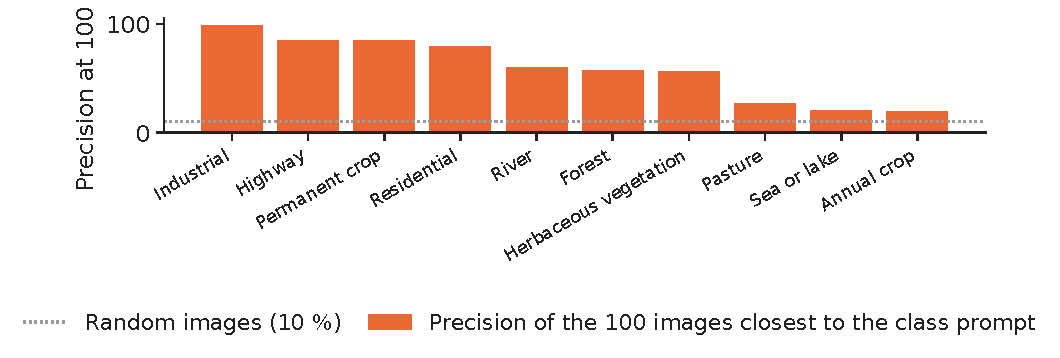
\includegraphics[width=\textwidth,height=0.332\textheight,keepaspectratio]{charts/en/text_search.pdf}\end{center}\vspace{-3mm}
\chartsource{Source: EuroSAT, Sentinel-2 images (Helber et al., 2019). Data: 5400 test images; model CLIP ViT-B/16, 5 templates.}
\vspace{0.5mm}
\begin{itemize}\setlength{\itemsep}{0pt}
  \item Mean precision of the top 100: 58.9\,\%
    \begin{itemize}\setlength{\itemsep}{0pt}
      \item Best industrial (99.0\,\%), worst annual crop (20.0\,\%).
    \end{itemize}
\end{itemize}
\par\vfill\manager{search first, label the hits, then train a probe: the cheapest way to build a labelled image set.}\par\vspace{0.5mm}
\par\vfill\noindent{\scriptsize\color{FooterGray}}\hfill\qlink{NN\_L14\_text\_search}{Quantlets/L14/NN_L14_text_search}\par\vspace{0.5mm}
\end{frame}

\begin{frame}{A linear probe: CLIP features plus logistic regression}
\footnotesize
\intuition{keep CLIP frozen and train only a logistic regression on its image embeddings.}
\begin{columns}[T,onlytextwidth]
\begin{column}{0.53\textwidth}
\[ \hat p(c\mid I)=\softmax\big(\mathbf W\mathbf u(I)+\mathbf b\big)_c \]\[ \min_{\mathbf W,\mathbf b}\ -\sum_{i}\log\hat p(c_i\mid I_i)+\frac{1}{2C}\lVert\mathbf W\rVert_F^2 \]{\footnotesize\begin{itemize}\setlength{\itemsep}{0pt}
  \item \textbf{\txtwhere}
    \begin{itemize}\setlength{\itemsep}{0pt}
      \item $\mathbf u(I)$ = normalised ViT-B/16 embedding (512 dimensions)
      \item $C=10$ fixed a priori
      \item $k$ labelled images per class, 5 seeds.
    \end{itemize}
\end{itemize}\par}
\end{column}
\begin{column}{0.44\textwidth}
\begin{itemize}\setlength{\itemsep}{2pt}
  \item \textbf{All training images}: 95.5\,\% (ViT-B/32: 94.8\,\%).
  \item \textbf{Beats zero-shot} already with one labelled image per class: 59.0\,\%.
\end{itemize}
\end{column}
\end{columns}
\par\vfill\manager{a probe trains in seconds on a laptop: the first thing to try when you have a few hundred labels.}\par\vspace{0.5mm}
\par\vfill\noindent{\scriptsize\color{FooterGray}}\hfill\tryit{notebook \S3}\par\vspace{0.5mm}
\end{frame}

\begin{frame}{Pre-trained features and a CNN trained from scratch, by number of labels}
\small
\intuition{one labelled image per class already beats zero-shot; from about 64 per class a small network trained from scratch catches up.}
\begin{center}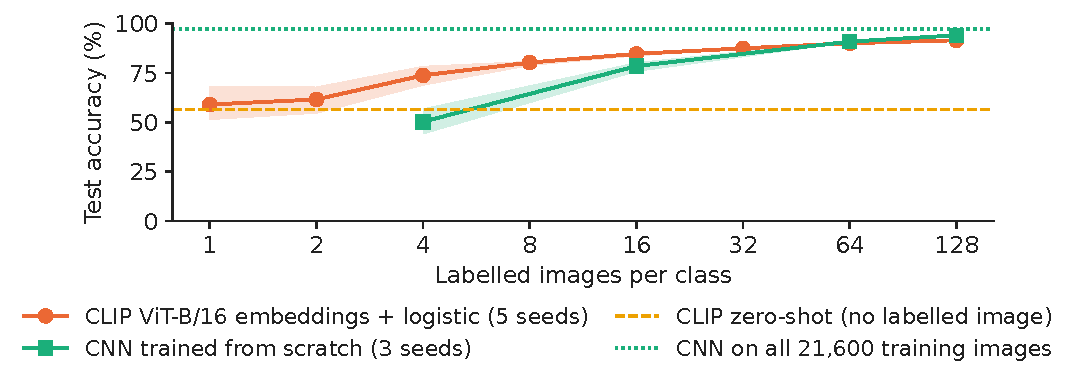
\includegraphics[width=\textwidth,height=0.331\textheight,keepaspectratio]{charts/en/fewshot_eurosat.pdf}\end{center}\vspace{-3mm}
\chartsource{Source: EuroSAT, Sentinel-2 images (Helber et al., 2019). Data: 5400 test images; shaded = range over seeds.}
\vspace{0.5mm}
\begin{itemize}\setlength{\itemsep}{0pt}
  \item 16 images per class: probe 84.7\,\%, convolutional neural network (CNN) 78.5\,\%
    \begin{itemize}\setlength{\itemsep}{0pt}
      \item 128 per class: 91.6\,\% vs 94.1\,\%
      \item All 21\,600 images: CNN 97.4\,\%, probe 95.5\,\%.
    \end{itemize}
\end{itemize}
\par\vfill\manager{with abundant labels a small CNN catches up
    \begin{itemize}\setlength{\itemsep}{0pt}
      \item With scarce labels, start from a foundation model.
    \end{itemize}}\par\vspace{0.5mm}
\par\vfill\noindent{\scriptsize\color{FooterGray}}\hfill\qlink{NN\_L14\_fewshot\_eurosat}{Quantlets/L14/NN_L14_fewshot_eurosat}\par\vspace{0.5mm}
\end{frame}

\begin{frame}{Size and speed of the three image models}
\small
{\footnotesize\renewcommand{\arraystretch}{1.05}\setlength{\tabcolsep}{4pt}
\begin{tabular}{@{}lrrr@{}}\toprule
Model & Parameters & ms per image & Test accuracy (\%) \\ \midrule
CNN from scratch (all labels) & 289.2 thousand & -- & 97.4 \\
CLIP ViT-B/32 + probe & 151.3 million & 4.23 & 94.8 \\
CLIP ViT-B/16 + probe & 149.6 million & 20.49 & 95.5 \\
Qwen2-VL-2B (chart questions) & 2.21 billion & 262 & -- \\
\bottomrule\end{tabular}}
\par\vspace{0.5mm}{\scriptsize \begin{itemize}\setlength{\itemsep}{0pt}
  \item Time measured on a laptop (Apple silicon graphics processor) for embedding one image in batches; the VLM time includes the question.
  \item A bigger patch (32 instead of 16 pixels) means 4 times fewer tokens: faster, slightly less accurate.
\end{itemize}}
\par\vfill\noindent{\scriptsize\color{FooterGray}(own computation)}\par\vspace{0.5mm}
\end{frame}


\section{Vision-language models: reading charts and tables}

\begin{frame}{A VLM plugs an image encoder into a language model}
\footnotesize
\intuition{image patches are projected into the word-embedding space of a large language model (LLM), which reads them as extra tokens.}
\begin{columns}[T,onlytextwidth]
\begin{column}{0.53\textwidth}
\[ \mathbf H_v=\mathbf W_p\,f_{\text{ViT}}(I) \]\[ p(y_t\mid y_{<t},I,q)=\mathrm{LLM}_{\btheta}\big([\mathbf H_v;\ \mathbf e(q);\ \mathbf e(y_{<t})]\big) \]{\footnotesize\begin{itemize}\setlength{\itemsep}{0pt}
  \item \textbf{\txtwhere}
    \begin{itemize}\setlength{\itemsep}{0pt}
      \item $f_{\text{ViT}}$ = vision encoder
      \item $\mathbf W_p$ = projector (an MLP)
      \item $q$ = question
      \item Trained first on image--caption pairs, then on visual instructions.
    \end{itemize}
\end{itemize}\par}
\end{column}
\begin{column}{0.44\textwidth}
\begin{itemize}\setlength{\itemsep}{2pt}
  \item \textbf{Large language and vision assistant (LLaVA)} introduced this recipe
    \begin{itemize}\setlength{\itemsep}{0pt}
      \item Qwen2-VL adds images of any resolution.
    \end{itemize}
  \item \textbf{Our model}: Qwen2-VL-2B-Instruct, 2.21 billion parameters, run locally.
\end{itemize}
\end{column}
\end{columns}
\par\vfill\manager{the answer is generated text: constrain it (yes/no, a number) and score it like a classifier.}\par\vspace{0.5mm}
\par\vfill\noindent{\scriptsize\color{FooterGray}(Liu et al., 2023; Wang et al., 2024)}\par\vspace{0.5mm}
\end{frame}

\begin{frame}{Market regimes as a visual recognition task}
\footnotesize
\intuition{draw the last 120 days of the S\&P 500 as an image and ask whether the market is in stress, as a chart analyst would.}
\begin{columns}[T,onlytextwidth]
\begin{column}{0.53\textwidth}
\[ S_t=\mathbb 1\Big\{\sigma^{(20)}_t>Q_{0.9}\big(\sigma^{(20)}_{t-750:t-1}\big)\Big\} \]\[ \sigma^{(20)}_t=\sqrt{252}\,\mathrm{sd}(r_{t-19:t}) \]{\footnotesize\begin{itemize}\setlength{\itemsep}{0pt}
  \item \textbf{\txtwhere}
    \begin{itemize}\setlength{\itemsep}{0pt}
      \item $S_t$ = stress label at the end of the window: 20-day volatility above its rolling 90th percentile of the previous three years (past data only)
      \item Windows every 5 days
      \item Train until 2018, test 394 windows from 2019.
    \end{itemize}
\end{itemize}\par}
\end{column}
\begin{column}{0.44\textwidth}
\begin{itemize}\setlength{\itemsep}{2pt}
  \item \textbf{Four readers of the same windows}
    \begin{itemize}\setlength{\itemsep}{0pt}
      \item Numbers + logistic regression (returns, volatility, drawdown)
      \item CLIP image embedding + logistic regression
      \item CLIP zero-shot: ``calm, steadily rising'' vs ``volatile, sharp crash''
      \item Qwen2-VL zero-shot: ``is the market turbulent?'' yes or no
    \end{itemize}
\end{itemize}
\end{column}
\end{columns}
\par\vfill\manager{a rolling-quantile label avoids hand-labelling and look-ahead.}\par\vspace{0.5mm}
\par\vfill\noindent{\scriptsize\color{FooterGray}(Jheng, Pele, Tak \& Găman, 2026)}\hfill\tryit{notebook \S4}\par\vspace{0.5mm}
\end{frame}

\begin{frame}{Detecting market stress from charts and from numbers}
\small
\intuition{left: a calm and a stress window as the models see them; right: receiver operating characteristic (ROC) curves on the test years.}
\begin{center}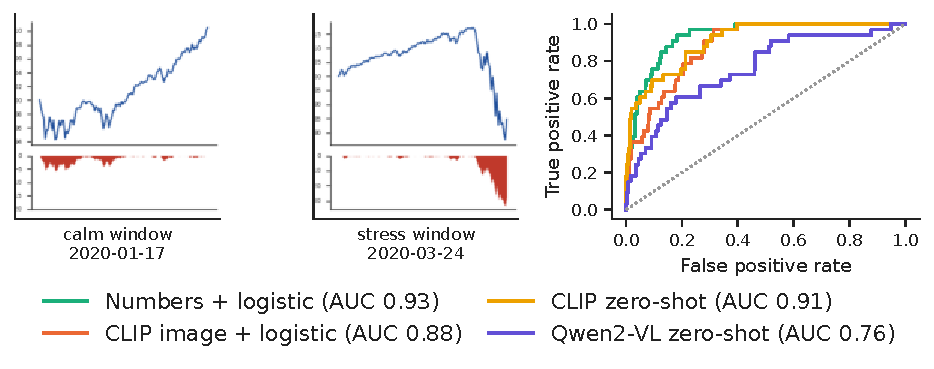
\includegraphics[width=\textwidth,height=0.469\textheight,keepaspectratio]{charts/en/chart_regime.pdf}\end{center}\vspace{-3mm}
\chartsource{Source: Yahoo Finance, daily quotes. Data: S\&P 500, windows of 120 trading days every 5 days; test 7 Jan 2019 to 30 Oct 2026.}
\vspace{0.5mm}
\begin{itemize}\setlength{\itemsep}{0pt}
  \item Area under the ROC curve (AUC): numbers 0.933, CLIP probe 0.880, CLIP zero-shot 0.907, Qwen2-VL zero-shot 0.758
    \begin{itemize}\setlength{\itemsep}{0pt}
      \item Stress share in test 8.4\,\%.
    \end{itemize}
\end{itemize}
\par\vfill\noindent{\scriptsize\color{FooterGray}}\hfill\qlink{NN\_L14\_chart\_regime}{Quantlets/L14/NN_L14_chart_regime}\par\vspace{0.5mm}
\end{frame}

\begin{frame}{Stress detection: discrimination and precision on the test years}
\small
\begin{columns}[T,onlytextwidth]
\begin{column}{0.5\textwidth}
{\scriptsize\renewcommand{\arraystretch}{1.05}\setlength{\tabcolsep}{4pt}
\begin{tabular}{@{}lrrl@{}}\toprule
Method & AUC & Avg.\ prec. & Labels \\ \midrule
Numbers + logistic & \cellcolor{Forest!55}0.933 & \cellcolor{Forest!49}0.578 & yes \\
CLIP image + logistic & \cellcolor{Forest!42}0.880 & \cellcolor{Forest!22}0.449 & yes \\
CLIP zero-shot & \cellcolor{Forest!48}0.907 & \cellcolor{Forest!55}0.605 & no \\
Qwen2-VL zero-shot & \cellcolor{Forest!11}0.758 & \cellcolor{Crimson!9}0.302 & no \\
\bottomrule\end{tabular}}
\end{column}
\begin{column}{0.47\textwidth}
\begin{itemize}\setlength{\itemsep}{4pt}
  \item \textbf{Best}: numbers.
  \item \textbf{Average precision} of a random score = stress share, 8.4\,\%.
  \item \textbf{Lesson}: when the numbers exist, a picture adds a lossy step
    \begin{itemize}\setlength{\itemsep}{0pt}
      \item Images earn their place when the numbers are missing (scans, screenshots, satellite).
    \end{itemize}
\end{itemize}
\end{column}
\end{columns}
\par\vfill\noindent{\scriptsize\color{FooterGray}(own computation, after Jheng, Pele, Tak \& Găman, 2026)}\hfill\tryit{notebook \S4}\par\vspace{0.5mm}
\end{frame}

\begin{frame}{What a 2-billion-parameter VLM can read: trends and table cells}
\small
\begin{itemize}\setlength{\itemsep}{3pt}
  \item \textbf{Trend question} on 394 test charts: ``did the price end higher or lower?''
    \begin{itemize}\setlength{\itemsep}{0pt}
      \item Accuracy 57.1\,\% at the 0.5 threshold, below always answering the majority (74.9\,\%)
      \item Yet AUC 0.974: the ranking is right, the threshold is biased --- recalibrate on validation charts
    \end{itemize}
  \item \textbf{Table question} on 60 ECB yield-curve tables: ``what is the 10-year yield?''
    \begin{itemize}\setlength{\itemsep}{0pt}
      \item Exact answers 25.0\,\%; mean absolute error 0.192 percentage points; numbers parsed 100.0\,\%
    \end{itemize}
  \item \textbf{Why it matters}
    \begin{itemize}\setlength{\itemsep}{0pt}
      \item Reading a cell is optical character recognition (OCR) plus locating the column: errors are silent and plausible
      \item For documents with known layout, extract the numbers with a parser and use the VLM only where layout varies
    \end{itemize}
\end{itemize}
\par\vfill\noindent{\scriptsize\color{FooterGray}(own computation; Wang et al., 2024)}\hfill\tryit{notebook \S5}\par\vspace{0.5mm}
\end{frame}

\begin{frame}{A document pipeline in a bank: where the VLM fits}
\small
\begin{itemize}\setlength{\itemsep}{3pt}
  \item \textbf{1. Capture}
    \begin{itemize}\setlength{\itemsep}{0pt}
      \item Scanned page or electronic file; known templates go to a rule-based parser
    \end{itemize}
  \item \textbf{2. Read}
    \begin{itemize}\setlength{\itemsep}{0pt}
      \item OCR and layout for text and tables; a VLM for free-form pages, charts and stamps
    \end{itemize}
  \item \textbf{3. Check}
    \begin{itemize}\setlength{\itemsep}{0pt}
      \item Totals must add up, dates must be valid, values within ranges; a failed check goes to a person
    \end{itemize}
  \item \textbf{4. Measure}
    \begin{itemize}\setlength{\itemsep}{0pt}
      \item Exact-match rate per field on a labelled sample, as for the yield tables (25.0\,\% here)
    \end{itemize}
\end{itemize}
\end{frame}

\begin{frame}{Capabilities and limitations of multimodal models}
\small
\begin{columns}[T,onlytextwidth]
\begin{column}{0.49\textwidth}
\begin{itemize}\setlength{\itemsep}{3pt}
  \item \textbf{Can}
    \begin{itemize}\setlength{\itemsep}{0pt}
      \item Label images with no training data (56.4\,\% on EuroSAT)
      \item Give features that need few labels (84.7\,\% with 16 per class)
      \item Search images by text, and text by images
      \item Answer simple questions about charts and documents
    \end{itemize}
\end{itemize}
\end{column}
\begin{column}{0.48\textwidth}
\begin{itemize}\setlength{\itemsep}{3pt}
  \item \textbf{Cannot (reliably)}
    \begin{itemize}\setlength{\itemsep}{0pt}
      \item Replace the numbers behind a chart
      \item Read every cell of a table correctly (25.0\,\% exact here)
      \item Explain faithfully why they answered
      \item Separate look-alike classes without examples
    \end{itemize}
\end{itemize}
\end{column}
\end{columns}
\par\vspace{0.5mm}{\scriptsize \begin{itemize}\setlength{\itemsep}{0pt}
  \item Controls: a labelled test set, constrained answers, human review of low-confidence cases, logs of every prompt and image.
\end{itemize}}
\end{frame}


\section{Synthesis of the course}

\begin{frame}{Methods of the course by data type}
\small
{\scriptsize\renewcommand{\arraystretch}{1.05}\setlength{\tabcolsep}{4pt}
\begin{tabular}{@{}p{0.2\textwidth}p{0.36\textwidth}p{0.37\textwidth}@{}}\toprule
Data & Models & Lectures and business cases \\ \midrule
Tables & logistic regression, MLP, regularisation & 1--3: credit scoring, fraud \\
Images & CNN, transfer learning, ViT, CLIP & 4, 14: land use, documents \\
Sequences & long short-term memory (LSTM), basis-expansion networks, foundation models & 5, 13: prices, load, Value-at-Risk (VaR) \\
Text & embeddings, transformers, LLM, retrieval-augmented generation (RAG) & 6, 7, 12: sentiment, central banks \\
Generation & variational autoencoder (VAE), generative adversarial network (GAN), diffusion & 8: synthetic data, anomalies \\
Graphs & graph neural network (GNN) & 9: transaction networks \\
Decisions & reinforcement learning (RL) & 10: trading, hedging, batteries \\
Trust & explainable artificial intelligence (XAI): Shapley additive explanations (SHAP), gradients & 11: credit audits \\
\bottomrule\end{tabular}}
\end{frame}

\begin{frame}{Choosing a model for a business problem}
\small
\begin{itemize}\setlength{\itemsep}{2pt}
  \item \textbf{1. Start with the decision and the cost of errors}
    \begin{itemize}\setlength{\itemsep}{0pt}
      \item A missed fraud and a false alarm do not cost the same; choose the metric before the model
    \end{itemize}
  \item \textbf{2. Fit the benchmark first}
    \begin{itemize}\setlength{\itemsep}{0pt}
      \item Logistic regression, the naive forecast, a Lasso autoregression, a volatility model, word counts with a linear classifier: minutes, interpretable
    \end{itemize}
  \item \textbf{3. Count your labels}
    \begin{itemize}\setlength{\itemsep}{0pt}
      \item Few labels: foundation model zero-shot or with a probe; many labels: a trained network
    \end{itemize}
  \item \textbf{4. Match the architecture to the data}
    \begin{itemize}\setlength{\itemsep}{0pt}
      \item Tables MLP or boosting, images CNN or ViT, sequences recurrent or transformer, graphs GNN
    \end{itemize}
  \item \textbf{5. Prove it}
    \begin{itemize}\setlength{\itemsep}{0pt}
      \item Test once, several seeds, a significance test, calibration, an explanation for the regulator
    \end{itemize}
\end{itemize}
\end{frame}

\begin{frame}{Five evaluation rules that held in every lecture}
\small
\begin{itemize}\setlength{\itemsep}{4pt}
  \item \textbf{No leakage}: scalers, prompts and thresholds are chosen on training or validation data
    \begin{itemize}\setlength{\itemsep}{0pt}
      \item Time series are split in time.
    \end{itemize}
  \item \textbf{A benchmark next to every network}: here, a CNN trained from scratch next to CLIP, numbers next to chart images.
  \item \textbf{Seeds and intervals}: the few-shot results above are means over 5 seeds with their range.
  \item \textbf{Metrics for rare events}: average precision and AUC for stress, not accuracy.
  \item \textbf{Real data, reproducible}: every number comes from a script and a public data set, with a Quantlet.
\end{itemize}
\end{frame}

\begin{frame}{Foundation models for images, text and time series}
\small
\begin{itemize}\setlength{\itemsep}{3pt}
  \item \textbf{The pattern}
    \begin{itemize}\setlength{\itemsep}{0pt}
      \item Pre-train once on huge unlabelled data; use zero-shot, with a few examples, or with a small trained head
    \end{itemize}
  \item \textbf{Text} (Lecture 12)
    \begin{itemize}\setlength{\itemsep}{0pt}
      \item Prompts and LLM embeddings for sentiment, RAG on ECB speeches, LLM-VaR
    \end{itemize}
  \item \textbf{Time series} (Lecture 13)
    \begin{itemize}\setlength{\itemsep}{0pt}
      \item Chronos-type models forecasting prices, load and VaR without training
    \end{itemize}
  \item \textbf{Images} (this lecture)
    \begin{itemize}\setlength{\itemsep}{0pt}
      \item CLIP zero-shot 56.4\,\%; probe on all labels 95.5\,\%
    \end{itemize}
  \item \textbf{The common caveat}
    \begin{itemize}\setlength{\itemsep}{0pt}
      \item Pre-training data may contain your test set; evaluate on data the model cannot have seen
    \end{itemize}
\end{itemize}
\end{frame}

\begin{frame}{Ten formulas of the course (1/2): learning}
\small
{\footnotesize\renewcommand{\arraystretch}{1.4}\setlength{\tabcolsep}{4pt}
\begin{tabular}{@{}p{0.27\textwidth}p{0.47\textwidth}p{0.18\textwidth}@{}}\toprule
Idea & Formula & Lecture \\ \midrule
Logistic neuron & $\hat p=\sigma(\mathbf w^{\top}\mathbf x+b)$ & 1 \\
Cross-entropy loss & $\loss=-\sum_i[y_i\log\hat p_i+(1-y_i)\log(1-\hat p_i)]$ & 1--2 \\
Backpropagation & $\boldsymbol\delta^{(\ell)}=(\mathbf W^{(\ell+1)\top}\boldsymbol\delta^{(\ell+1)})\odot f'(\mathbf z^{(\ell)})$ & 2 \\
Gradient step (Adam without moments) & $\btheta\leftarrow\btheta-\eta\nabla_{\btheta}\loss$ & 2 \\
Weight decay & $\loss+\lambda\lVert\btheta\rVert_2^2$ & 3 \\
\bottomrule\end{tabular}}
\par\vspace{0.5mm}{\scriptsize \begin{itemize}\setlength{\itemsep}{0pt}
  \item All symbols as defined in the lectures cited; $\sigma$ = logistic function, $\odot$ = element-wise product.
\end{itemize}}
\end{frame}

\begin{frame}{Ten formulas of the course (2/2): architectures}
\small
{\footnotesize\renewcommand{\arraystretch}{1.4}\setlength{\tabcolsep}{4pt}
\begin{tabular}{@{}p{0.27\textwidth}p{0.47\textwidth}p{0.18\textwidth}@{}}\toprule
Idea & Formula & Lecture \\ \midrule
Convolution & $(\mathbf K*\mathbf X)_{ij}=\sum_{u,v}K_{uv}X_{i+u,j+v}$ & 4 \\
Recurrent state & $\mathbf h_t=\tanh(\mathbf W\mathbf h_{t-1}+\mathbf U\mathbf x_t+\mathbf b)$ & 5 \\
Attention & $\softmax(\mathbf Q\mathbf K^{\top}/\sqrt{d_k})\mathbf V$ & 7, 12--14 \\
Graph convolution & $\mathbf H'=\sigma(\tilde{\mathbf D}^{-1/2}\tilde{\mathbf A}\tilde{\mathbf D}^{-1/2}\mathbf H\mathbf W)$ & 9 \\
Contrastive image--text loss & $-\log\frac{e^{s_{ii}}}{\sum_j e^{s_{ij}}}$ & 14 \\
\bottomrule\end{tabular}}
\par\vspace{0.5mm}{\scriptsize \begin{itemize}\setlength{\itemsep}{0pt}
  \item $\mathbf K$ = kernel; $\tilde{\mathbf A}$ = adjacency matrix with self-loops, $\tilde{\mathbf D}$ its degree matrix; $s_{ij}$ = scaled image--text similarity.
\end{itemize}}
\end{frame}

\begin{frame}{Responsible use: the same rules for every model of the course}
\small
\begin{itemize}\setlength{\itemsep}{3pt}
  \item \textbf{Regulation}
    \begin{itemize}\setlength{\itemsep}{0pt}
      \item The European Union Artificial Intelligence Act (Regulation 2024/1689) lists credit scoring among high-risk uses: documentation, human oversight, data governance
    \end{itemize}
  \item \textbf{Documentation}
    \begin{itemize}\setlength{\itemsep}{0pt}
      \item A model card: data, period, metric, benchmark, seeds, known failure cases (here: sea or lake read as highway)
    \end{itemize}
  \item \textbf{Monitoring}
    \begin{itemize}\setlength{\itemsep}{0pt}
      \item Re-test on new data: price regimes, new satellite seasons, new speech topics
    \end{itemize}
  \item \textbf{Privacy}
    \begin{itemize}\setlength{\itemsep}{0pt}
      \item Local open models keep client documents and images in-house
    \end{itemize}
\end{itemize}
\end{frame}

\begin{frame}{What a good course project looks like}
\small
\begin{columns}[T,onlytextwidth]
\begin{column}{0.49\textwidth}
\begin{itemize}\setlength{\itemsep}{3pt}
  \item \textbf{Question and data}
    \begin{itemize}\setlength{\itemsep}{0pt}
      \item One business decision, one public data set, its period and licence
    \end{itemize}
  \item \textbf{Benchmark first}
    \begin{itemize}\setlength{\itemsep}{0pt}
      \item A linear or naive model, reported next to every network
    \end{itemize}
  \item \textbf{Leakage check}
    \begin{itemize}\setlength{\itemsep}{0pt}
      \item Time-ordered split, scalers fitted on training data, test used once
    \end{itemize}
\end{itemize}
\end{column}
\begin{column}{0.48\textwidth}
\begin{itemize}\setlength{\itemsep}{3pt}
  \item \textbf{Uncertainty}
    \begin{itemize}\setlength{\itemsep}{0pt}
      \item Several seeds, bootstrap intervals or a Diebold--Mariano test
    \end{itemize}
  \item \textbf{Explanation}
    \begin{itemize}\setlength{\itemsep}{0pt}
      \item SHAP or gradients for the decision that matters
    \end{itemize}
  \item \textbf{Reproducible}
    \begin{itemize}\setlength{\itemsep}{0pt}
      \item One script from raw data to every number and chart
    \end{itemize}
\end{itemize}
\end{column}
\end{columns}
\end{frame}

\begin{frame}{Open research problems for dissertations}
\small
\begin{columns}[T,onlytextwidth]
\begin{column}{0.49\textwidth}
\begin{itemize}\setlength{\itemsep}{4pt}
  \item \textbf{Calibration under drift}: conformal bands that stay valid when markets change regime.
  \item \textbf{Leakage-proof evaluation} of foundation models trained on the open web.
  \item \textbf{Stable explanations}: do SHAP values of a credit model survive a retraining?
\end{itemize}
\end{column}
\begin{column}{0.48\textwidth}
\begin{itemize}\setlength{\itemsep}{4pt}
  \item \textbf{Small models for small institutions}: when does a 2--3 billion model on a laptop suffice?
  \item \textbf{Multimodal risk signals}: satellite, text and prices in one early-warning model.
  \item \textbf{Romanian data}: language models and forecasts for Romanian text, markets and energy.
\end{itemize}
\end{column}
\end{columns}
\end{frame}

\section*{Wrap-up}

\begin{frame}{Quiz 1: zero-shot classifier}
\small
\begin{itemize}
  \item A bank wants to flag flooded fields in satellite images but has no labelled flood image
    \begin{itemize}\setlength{\itemsep}{0pt}
      \item What can it do with CLIP?
    \end{itemize}
\end{itemize}
\vspace{2mm}
\begin{exampleblock}{Answer}
\begin{itemize}
  \item Write class prompts (``a satellite photo of a flooded field'', ``\ldots{} of a dry field''), embed them and classify by cosine similarity
    \begin{itemize}\setlength{\itemsep}{0pt}
      \item Then label a few hundred images to validate and train a probe.
    \end{itemize}
\end{itemize}
\end{exampleblock}
\end{frame}

\begin{frame}{Quiz 2: pictures or numbers}
\small
\begin{itemize}
  \item Why did the numeric logistic model detect market stress at least as well as models reading the chart image?
\end{itemize}
\vspace{2mm}
\begin{exampleblock}{Answer}
\begin{itemize}
  \item The image is drawn from the same numbers, with resolution lost
    \begin{itemize}\setlength{\itemsep}{0pt}
      \item The numbers carry the volatility directly.
      \item Images help when no numbers exist.
    \end{itemize}
\end{itemize}
\end{exampleblock}
\end{frame}

\begin{frame}{Quiz 3: labels}
\small
\begin{itemize}
  \item With 16 labelled images per class, which do you choose: a CNN from scratch or a probe on CLIP embeddings?
\end{itemize}
\vspace{2mm}
\begin{exampleblock}{Answer}
\begin{itemize}
  \item The probe: 84.7\,\% against 78.5\,\% for the CNN on our data.
\end{itemize}
\end{exampleblock}
\end{frame}

\begin{frame}{Wrap-up}
\small
\begin{itemize}\setlength{\itemsep}{4pt}
  \item A ViT reads images as patch tokens
    \begin{itemize}\setlength{\itemsep}{0pt}
      \item CLIP aligns them with text by a contrastive loss.
    \end{itemize}
  \item Zero-shot CLIP labels satellite images at 56.4\,\% with no labels
    \begin{itemize}\setlength{\itemsep}{0pt}
      \item A probe reaches 95.5\,\%.
    \end{itemize}
  \item VLMs answer questions about charts and tables, but must be scored like any classifier.
  \item The course in one line: benchmark first, real data, no leakage, several seeds, a test, an explanation.
\end{itemize}
\end{frame}

\begin{frame}{Research from our group}
\footnotesize
\begin{itemize}\setlength{\itemsep}{3pt}
  \item \textbf{Multimodal vision-language anomaly detection} (Best Paper Award, International Conference on Business Excellence (ICBE) 2026): market indicators are projected onto multi-panel images, a VLM (GPT-4.1, generative pre-trained transformer) classifies the regime zero-shot with rolling-quantile labels and explains its choice
    \begin{itemize}\setlength{\itemsep}{0pt}
      \item Validated out of sample on the S\&P 500 (Jheng, Pele, Tak \& Găman, 2026, PICBE).
    \end{itemize}
  \item \textbf{Explainable fraud detection}: tabular models and graph networks combined with SHAP and graph ablation (Diaconu \& Pele, 2026, PICBE) --- Case study 1.
  \item \textbf{LLM-VaR and LLM-ES}: language models as zero-shot risk models (Pele et al., 2026, Expert Systems with Applications) --- Lectures 12 and 13.
  \item \textbf{ESG-aware portfolios}: multi-criteria selection of assets with ESG scores (Găman, Tak, Jheng \& Pele, 2026, PICBE).
\end{itemize}
\par\vspace{0.5mm}{\scriptsize \begin{itemize}\setlength{\itemsep}{0pt}
  \item Findings as stated in the papers' abstracts; numbers on the other slides come from our own data.
\end{itemize}}
\par\vfill\noindent{\scriptsize\color{FooterGray}(Bucharest University of Economic Studies, ASE; Romanian Academy, Institute for Economic Forecasting, IPE)}\par\vspace{0.5mm}
\end{frame}

\begin{frame}{Further reading and resources}
\small
\begin{columns}[T,onlytextwidth]
\begin{column}{0.5\textwidth}
\begin{itemize}\setlength{\itemsep}{4pt}
  \item \textbf{OpenCLIP} models and benchmarks: \href{https://github.com/mlfoundations/open_clip}{github.com/mlfoundations/open\_clip}.
  \item \textbf{Qwen2-VL}: \href{https://github.com/QwenLM/Qwen2-VL}{github.com/QwenLM/Qwen2-VL}.
  \item \textbf{Bishop \& Bishop (2024)}, chapters 12 and 20: \href{https://www.bishopbook.com}{bishopbook.com}.
\end{itemize}
\end{column}
\begin{column}{0.47\textwidth}
\begin{itemize}\setlength{\itemsep}{4pt}
  \item \textbf{Quantinar}: Digital Transformation on Finance: \href{https://quantinar.com/course/674/digital-transformation-on-finance}{quantinar.com}.
  \item \textbf{EuroSAT} data: \href{https://github.com/phelber/EuroSAT}{github.com/phelber/EuroSAT}.
  \item \textbf{This lecture}: notebook, seminar and Quantlets --- \href{https://github.com/danpele/NEURAL_BIZ}{github.com/danpele/NEURAL\_BIZ}.
\end{itemize}
\end{column}
\end{columns}
\end{frame}

\begin{frame}{References (1/2)}
\scriptsize
\begin{itemize}\setlength{\itemsep}{0pt}\scriptsize
\item Abnar, S.\ \& Zuidema, W.\ (2020). Quantifying attention flow in transformers. \textit{Proceedings of the 58th Annual Meeting of the Association for Computational Linguistics}, 4190--4197. \href{https://doi.org/10.18653/v1/2020.acl-main.385}{doi:10.18653/v1/2020.acl-main.385}
\item Bishop, C.\,M.\ \& Bishop, H.\ (2024). \textit{Deep Learning: Foundations and Concepts}. Springer. \href{https://doi.org/10.1007/978-3-031-45468-4}{doi:10.1007/978-3-031-45468-4}
\item Diaconu, D.\ \& Pele, D.\,T.\ (2026). Explainable AI in financial fraud detection: Evidence from the IEEE-CIS fraud dataset. \textit{Proceedings of the International Conference on Business Excellence}, 20(1), 118--132. \href{https://doi.org/10.2478/picbe-2026-0015}{doi:10.2478/picbe-2026-0015}
\item Dosovitskiy, A.\ et al.\ (2021). An image is worth 16x16 words: Transformers for image recognition at scale. \textit{International Conference on Learning Representations}. \href{https://arxiv.org/abs/2010.11929}{arXiv:2010.11929}
\item Găman, Ș., Tak, R., Jheng, S.-L.\ \& Pele, D.\,T.\ (2026). ESG-aware asset selection and portfolio optimization: A comparative study of multi-criteria decision-making methods. \textit{Proceedings of the International Conference on Business Excellence}, 20(1), 133--147. \href{https://doi.org/10.2478/picbe-2026-0016}{doi:10.2478/picbe-2026-0016}
\item Helber, P., Bischke, B., Dengel, A.\ \& Borth, D.\ (2019). EuroSAT: A novel dataset and deep learning benchmark for land use and land cover classification. \textit{IEEE Journal of Selected Topics in Applied Earth Observations and Remote Sensing}, 12(7), 2217--2226. \href{https://doi.org/10.1109/JSTARS.2019.2918242}{doi:10.1109/JSTARS.2019.2918242}
\item Jheng, S.-L., Pele, D.\,T., Tak, R.\ \& Găman, Ș.\ (2026). A multimodal vision-language framework for financial anomaly detection. \textit{Proceedings of the International Conference on Business Excellence}, 20(1), 191--201. \href{https://doi.org/10.2478/picbe-2026-0020}{doi:10.2478/picbe-2026-0020}
\end{itemize}
\end{frame}

\begin{frame}{References (2/2)}
\scriptsize
\begin{itemize}\setlength{\itemsep}{0pt}\scriptsize
\item Liu, H., Li, C., Wu, Q.\ \& Lee, Y.\,J.\ (2023). Visual instruction tuning. \textit{Advances in Neural Information Processing Systems}, 36. \href{https://arxiv.org/abs/2304.08485}{arXiv:2304.08485}
\item Oord, A.\ van den, Li, Y.\ \& Vinyals, O.\ (2018). Representation learning with contrastive predictive coding. \href{https://arxiv.org/abs/1807.03748}{arXiv:1807.03748}
\item Pele, D.\,T., Bolovăneanu, V., Lin, M.-B., Ren, R., Ginavar, A.\,T., Spilak, B., Andrei, A.-V., Toma, F.-M., Lessmann, S.\ \& Härdle, W.\,K.\ (2026). In the beginning was the Word: LLM-VaR and LLM-ES. \textit{Expert Systems with Applications}, 295, 128676. \href{https://doi.org/10.1016/j.eswa.2025.128676}{doi:10.1016/j.eswa.2025.128676}
\item Radford, A.\ et al.\ (2021). Learning transferable visual models from natural language supervision. \textit{Proceedings of the 38th International Conference on Machine Learning}, 8748--8763. \href{https://arxiv.org/abs/2103.00020}{arXiv:2103.00020}
\item Wang, P.\ et al.\ (2024). Qwen2-VL: Enhancing vision-language model's perception of the world at any resolution. \href{https://arxiv.org/abs/2409.12191}{arXiv:2409.12191}
\end{itemize}
\end{frame}

\appendix

\section*{Appendix}

\begin{frame}{Appendix A: the contrastive loss as a classification problem}
\small
\begin{itemize}\setlength{\itemsep}{4pt}
  \item Row $i$ of $\mathbf S=(s_{ij})$ is a softmax classifier over $n$ captions with the correct class $i$: the loss is cross-entropy with labels $0,\dots,n-1$.
  \item A larger batch means more negatives and a harder task
    \begin{itemize}\setlength{\itemsep}{0pt}
      \item CLIP used $n$ = 32,768.
    \end{itemize}
  \item Zero-shot classification is the same computation with the $n$ captions replaced by the $C$ class prompts.
\end{itemize}
\par\vfill\noindent{\scriptsize\color{FooterGray}(Radford et al., 2021; Oord et al., 2018)}\par\vspace{0.5mm}
\end{frame}

\begin{frame}{Appendix B: implementation details}
\small
\begin{itemize}\setlength{\itemsep}{4pt}
  \item CLIP: openai/clip-vit-base-patch32 and -patch16 (Hugging Face transformers), images resized to 224 pixels
    \begin{itemize}\setlength{\itemsep}{0pt}
      \item Logistic regression from scikit-learn.
    \end{itemize}
  \item CNN: three convolution blocks (32, 64, 128 channels), AdamW with a one-cycle schedule, flips and rotations as augmentation
    \begin{itemize}\setlength{\itemsep}{0pt}
      \item 289.2 thousand parameters.
    \end{itemize}
  \item VLM: Qwen/Qwen2-VL-2B-Instruct, float16
    \begin{itemize}\setlength{\itemsep}{0pt}
      \item Yes/no answers scored by first-token probabilities
      \item Numbers by greedy decoding.
    \end{itemize}
  \item Seed 20261108
    \begin{itemize}\setlength{\itemsep}{0pt}
      \item The full analysis ran in 0.6 minutes on its last run (embeddings and answers cached).
    \end{itemize}
\end{itemize}
\end{frame}

\end{document}
